\documentclass[10.5pt,a4paper]{article}
% ---------------------------------------------------------------------------
% Informe final - DataForge Consulting - Proyecto integrador DIBA
% Compilar desde la carpeta informe/:  python generar_anexos.py && pdflatex informe_final.tex (dos veces)
% ---------------------------------------------------------------------------
\usepackage[T1]{fontenc}
\usepackage[utf8]{inputenc}
\usepackage[spanish,es-noshorthands,es-tabla]{babel}
\usepackage{lmodern}
\usepackage[a4paper,top=2.1cm,bottom=2.1cm,left=2.2cm,right=2.2cm,headheight=14pt]{geometry}
\usepackage{graphicx,booktabs,tabularx,longtable,array,multirow,makecell,float}
\usepackage[table]{xcolor}
\usepackage{fancyhdr,titlesec,enumitem,microtype}
\usepackage[font=small,labelfont=bf,skip=4pt]{caption}
\usepackage[most]{tcolorbox}
\usepackage{tikz}
\usetikzlibrary{positioning,arrows.meta}
\usepackage[hidelinks]{hyperref}

\DeclareUnicodeCharacter{2265}{\ensuremath{\geq}}
\DeclareUnicodeCharacter{2264}{\ensuremath{\leq}}
\DeclareUnicodeCharacter{00D7}{\ensuremath{\times}}
\DeclareUnicodeCharacter{2212}{\ensuremath{-}}
\DeclareUnicodeCharacter{2192}{\ensuremath{\rightarrow}}
\DeclareUnicodeCharacter{2248}{\ensuremath{\approx}}
\DeclareUnicodeCharacter{03A3}{\ensuremath{\Sigma}}
\DeclareUnicodeCharacter{2260}{\ensuremath{\neq}}
\DeclareUnicodeCharacter{21D4}{\ensuremath{\Leftrightarrow}}

\definecolor{azul}{HTML}{1C5CAB}
\definecolor{azulclaro}{HTML}{CDE2FB}
\definecolor{naranja}{HTML}{EB6834}
\definecolor{gris}{HTML}{52514E}
\definecolor{grisclaro}{HTML}{F6F5F2}
\definecolor{critico}{HTML}{D03B3B}

\graphicspath{{../outputs/figuras/}}
\setlength{\parindent}{0pt}
\setlength{\parskip}{4pt}
\renewcommand{\arraystretch}{1.12}
\setlist{nosep,leftmargin=1.2em}
\titleformat{\section}{\large\bfseries\color{azul}}{\thesection.}{0.5em}{}
\titleformat{\subsection}{\normalsize\bfseries\color{azul}}{\thesubsection}{0.5em}{}
\titlespacing*{\section}{0pt}{10pt}{4pt}
\titlespacing*{\subsection}{0pt}{7pt}{2pt}
\pagestyle{fancy}
\fancyhf{}
\fancyhead[L]{\small\color{gris}DataForge Consulting · Proyecto final DIBA}
\fancyhead[R]{\small\color{gris}Telco: sistema de decisión para la retención}
\fancyfoot[C]{\small\thepage}
\renewcommand{\headrulewidth}{0.4pt}

\newtcolorbox{caja}[1][]{colback=grisclaro,colframe=azul,boxrule=0.6pt,arc=2pt,left=6pt,right=6pt,top=4pt,bottom=4pt,#1}
\renewcommand{\tabularxcolumn}[1]{>{\raggedright\arraybackslash}p{#1}}
\newcolumntype{P}[1]{>{\raggedright\arraybackslash}p{#1}}
\newcommand{\fuente}[1]{\par\vspace{-2pt}{\footnotesize\color{gris}#1}}

\begin{document}

% ===========================================================================
% PORTADA
% ===========================================================================
\begin{titlepage}
\thispagestyle{empty}
\vspace*{0.4cm}
{\color{azul}\rule{\textwidth}{1.2pt}}\\[4pt]
{\large\bfseries\color{azul} DataForge Consulting}\\[-2pt]
{\small\color{gris} Analítica para decidir mejor}\\[2.2cm]

{\Huge\bfseries Sistema de Decision Intelligence\\[4pt] para la retención de clientes}\\[10pt]
{\Large Caso Telco: qué clientes intervenir, con qué palanca y con qué retorno}\\[1.2cm]

{\large Informe final del proyecto integrador}\\[4pt]
Decision Intelligence \& Business Analytics · Maestría en Ciencia de Datos\\
Escuela Colombiana de Ingeniería Julio Garavito\\
Docente: Juliana De Mier Medellín\\[1.4cm]

\begin{caja}
\textbf{Pregunta de decisión.} ¿Qué segmentos de clientes activos debe priorizar la Gerencia de Retención este mes, con qué palanca de retención y con qué retorno esperado, para reducir el MRR perdido por churn sin deteriorar el ARPU?
\end{caja}
\vspace{1.0cm}

\textbf{Equipo consultor}\\[2pt]
Oscar Santiago Merino Suárez\\
Claudia Rocío Rodríguez Ortiz\\
Paula Andrea Gacha García\\
Daniel Felipe Pérez Pineda\\[1.2cm]

{\small\color{gris}
\textbf{Entregables que acompañan este informe:} notebook reproducible \texttt{notebooks/DataForge\_Telco\_Churn.ipynb} · dashboard Power BI \texttt{powerbi/DataForge\_Telco\_Churn.pbip} · diccionario de métricas \texttt{docs/diccionario\_metricas.md} · presentación ejecutiva \texttt{presentacion/} · \texttt{README.md}.}

\vfill
{\color{azul}\rule{\textwidth}{0.6pt}}\\
Bogotá, octubre de 2026
\end{titlepage}

% ===========================================================================
\section{Resumen ejecutivo}
% ===========================================================================
Telco perdió en el período de corte al \textbf{26.5\,\%} de sus clientes (1,869 de 7,043). Esos clientes pagaban \textbf{USD 139 mil al mes, el 30.5\,\% del ingreso recurrente mensual (MRR)}. DataForge Consulting diseñó un sistema de decisión que conecta ese problema con una decisión mensual: \emph{a qué clientes activos intervenir, con qué palanca y con cuánto presupuesto}. El sistema reúne un sistema de métricas con North Star, una tabla analítica auditada, un análisis de drivers, un simulador de ROI y un dashboard de monitoreo.

\textbf{Hallazgos principales}
\begin{itemize}
  \item \textbf{La pérdida está concentrada.} Los clientes \emph{mes a mes con fibra óptica} son el 30\,\% de la base, pero explican el 72\,\% del MRR perdido. Todo el contrato mes a mes explica el 87\,\%.
  \item \textbf{El riesgo vive en los primeros meses.} El churn es de 52.9\,\% entre 0 y 6 meses de antigüedad y de 9.5\,\% después de 49 meses. El patrón se mantiene dentro de cada tipo de contrato.
  \item \textbf{Drivers ajustados.} Contrato, antigüedad temprana, fibra (OR 2.1) y cheque electrónico (OR 1.4) aumentan el riesgo. La seguridad online y el soporte técnico lo reducen (OR $\approx$ 0.7).
  \item \textbf{Se pierden los clientes más valiosos.} Quienes abandonan pagan USD 74 al mes frente a USD 61 de los activos. Por eso la North Star pondera por valor: \textbf{\% MRR retenido = 69.5\,\%}.
\end{itemize}

\begin{caja}
\textbf{Recomendación.} \textbf{No} lanzar un descuento masivo a los clientes mes a mes: su ROI estimado es negativo en el escenario base (−32\,\%). Lanzar un \textbf{programa focalizado} sobre los \textbf{820 clientes activos de riesgo alto} (score $\geq$ 40\,\%; USD 64 mil de MRR), cada uno con una palanca asignada. Las palancas son onboarding temprano, bundle de protección, pago automático y, solo de forma residual, migración a contrato anual. El ROI estimado es de \textbf{+179\,\% en el escenario base y −48\,\% en el conservador}. Por eso el programa se ejecuta como \textbf{piloto con grupo control} y se escala solo si la reducción atribuible del riesgo supera el umbral de equilibrio (≈ 5\,\% con un horizonte de 12 meses).
\end{caja}

\textbf{Riesgos.} Hay un único corte sin fechas calendario, el churn está sobrerrepresentado en el dataset y la ventana del churn es ambigua. Además, el efecto de las palancas sale de asociaciones observacionales y los costos son supuestos. Todo esto se gestiona con escenarios, umbrales explícitos y el piloto A/B.

% ===========================================================================
\section{Contexto del negocio y problema}
% ===========================================================================
\textbf{Telco} es una operadora de telefonía e internet residencial que vive de suscripciones mensuales. Los datos provienen del caso público de IBM, así que la compañía es ficticia. En el corte analizado tiene 7,043 clientes con un MRR de USD 456 mil. Como supuesto del caso, la Gerencia de Retención reacciona al churn con ofertas genéricas de descuento: no prioriza a quién contactar, no distingue qué palanca usar con cada perfil y no mide el retorno de lo que hace.

Siguiendo el marco Data-to-Decision (Sesión 1), reformulamos el encargo. La formulación débil, \emph{``queremos un dashboard de churn''}, pasa a ser una formulación orientada a decisión: \emph{``la Gerencia de Retención necesita decidir cada mes qué segmentos de clientes activos intervenir, con qué palanca y con cuánto presupuesto, porque el churn se lleva un tercio del MRR''}. Es una decisión de nivel \textbf{táctico}: la toma la gerencia cada mes, con un componente \textbf{operativo} semanal (lista de contacto) y un KPI \textbf{estratégico} (\% MRR retenido) que el Comité Directivo revisa cada trimestre.

\textbf{Por qué importa.} Cada punto de churn evitado en los segmentos críticos protege un MRR superior al promedio. Además, una mala elección de palanca puede retener clientes a costa de destruir ARPU, por ejemplo con descuentos a clientes que no se iban a ir. El problema no es solo \emph{cuánto} churn hay, sino \emph{dónde} intervenir para que la acción sea rentable.

% ===========================================================================
\section{Decisión que se busca apoyar}
% ===========================================================================
\begin{table}[H]
\centering\footnotesize
\caption{Decision Canvas (Plantilla 1 del enunciado).}
\begin{tabularx}{\textwidth}{@{}>{\bfseries}P{3.1cm}X@{}}
\toprule
Problema organizacional & Pérdida de clientes y de ingreso recurrente por churn: 26.5\,\% de los clientes y 30.5\,\% del MRR en el corte, con acciones de retención genéricas y no priorizadas. \\
Objetivo de negocio & Reducir el MRR perdido por churn del 30.5\,\% al 25\,\% del MRR en dos trimestres sin que el ARPU caiga más de 3\,\% (balance). \\
Usuario de la decisión & Gerente de Retención y Experiencia del Cliente (decide). Audiencia ejecutiva: Comité Directivo (VP Comercial, CFO). Ejecutan: Customer Success, Facturación y Producto. \\
Decisión principal & Cada mes, qué segmentos de clientes activos intervenir, con qué palanca y con cuánto presupuesto. \\
Alternativas de acción & \textbf{A)} No intervenir. \textbf{B)} Descuento masivo a todos los clientes mes a mes. \textbf{C)} Programa focalizado por riesgo y valor con una palanca por perfil: L4 onboarding temprano, L2 bundle de protección, L3 pago automático, L1 migración a contrato anual. \textbf{D)} Revisión estructural de la propuesta de valor de la fibra (precio y calidad). \\
Frecuencia de decisión & Mensual (segmentos y presupuesto); seguimiento semanal de la ejecución; revisión trimestral de impacto con el Comité. \\
Métricas clave & North Star \% MRR retenido; tasa de churn; MRR perdido; churn temprano (0–6 m); \% contrato a plazo; \% pago automático; adopción de protección; ARPU y ROI del programa (balance). \\
Preguntas analíticas & ¿Dónde se concentra el MRR perdido? ¿Qué factores explican el churn? ¿Qué clientes activos combinan alto riesgo y alto valor? ¿Qué palanca tiene mejor retorno esperado y bajo qué supuestos? \\
Fuentes de datos & Telco Customer Churn (IBM/Kaggle): un corte con 7,043 clientes y 21 variables. A futuro: cortes mensuales, CRM de campañas y costos reales. \\
Unidad de análisis & Cliente: una fila por cliente en el corte. \\
Criterio de éxito & \% MRR perdido $\leq$ 25\,\%; uplift del piloto significativo frente al grupo control; ROI $\geq$ 0 en el escenario base; ARPU sin caídas mayores al 3\,\%. \\
Riesgos o sesgos & Snapshot sin fechas; ventana del churn ambigua; sesgo de selección en comparaciones observacionales; sesgo de supervivencia en la antigüedad; supuestos de costo y efecto. \\
Acción esperada & Piloto con grupo control sobre los clientes activos de riesgo alto, cada uno con su palanca; escalar solo si el uplift supera el umbral de equilibrio. \\
Monitoreo posterior & Dashboard mensual con semáforos (sección 12), lectura del piloto a 30, 60 y 90 días y guardrails de ARPU y costo. \\
\bottomrule
\end{tabularx}
\end{table}

% ===========================================================================
\section{Descripción del dataset y fuente}
% ===========================================================================
Trabajamos en la \textbf{Modalidad B} (dataset público). El dataset es \textbf{Telco Customer Churn} de IBM Sample Data Sets, publicado en Kaggle por \emph{blastchar} (\url{https://www.kaggle.com/datasets/blastchar/telco-customer-churn}). Es una sola tabla con \textbf{7,043 filas y 21 columnas}: identificador del cliente, perfil demográfico (género, adulto mayor, pareja, dependientes), antigüedad en meses (\emph{tenure}), servicios contratados (telefonía, líneas múltiples, tipo de internet y seis complementos), condiciones de cuenta (contrato, factura electrónica, método de pago), cargos (mensual y acumulado) y la marca de abandono (\emph{Churn}).

\begin{table}[H]
\centering\footnotesize
\caption{Condiciones mínimas del dataset (sección 4 del enunciado).}
\begin{tabularx}{\textwidth}{@{}lXl@{}}
\toprule
Requisito & Evidencia en Telco & ¿Cumple? \\
\midrule
Variable de fecha o período & No hay fecha calendario; \emph{tenure} (0–72 meses) permite análisis de ciclo de vida y cohortes por antigüedad & Parcial (justificado) \\
Identificador principal & \texttt{customerID}: único y sin nulos & Sí \\
Variable numérica & \texttt{MonthlyCharges} (MRR), \texttt{TotalCharges}, \texttt{tenure} & Sí \\
Variable categórica & Contrato, internet, método de pago, complementos, demografía & Sí \\
Variable de resultado & \texttt{Churn} (Yes/No) & Sí \\
Tamaño suficiente & 7,043 filas ($>$ 500) & Sí \\
Potencial de decisión & Las variables son palancas accionables (contrato, pago, servicios) & Sí \\
\bottomrule
\end{tabularx}
\end{table}

\textbf{Limitaciones iniciales.} (1) Es un único corte sin fechas: no hay serie mensual ni estacionalidad. (2) La ventana de churn es ambigua: Kaggle la describe como el ``último mes'' y la documentación extendida de IBM como el trimestre. (3) No hay costos, márgenes, campañas ni interacciones de soporte. (4) Los datos son sintéticos y didácticos. El alcance se ajusta en consecuencia: las conclusiones se apoyan en comparaciones relativas entre segmentos y los montos económicos se presentan con supuestos explícitos.

% ===========================================================================
\section{Unidad de análisis y granularidad}
% ===========================================================================
\begin{table}[H]
\centering\footnotesize
\caption{Mapa de granularidad.}
\begin{tabularx}{\textwidth}{@{}>{\bfseries}P{4.2cm}X@{}}
\toprule
Qué representa una fila & Un \textbf{cliente en un corte} (snapshot). Es una entidad, no un evento: 7,043 filas y 7,043 \texttt{customerID} únicos. \\
Granularidad (captura → análisis → reporte) & Cliente → \textbf{cliente-corte} (\texttt{df\_analitico}) → segmento y mes en el dashboard. \\
ID de entidad / ID de evento & \texttt{customer\_id} / no existe (no hay transacciones). \\
Fecha principal & No existe. El eje temporal es la \textbf{antigüedad} (meses de vida del cliente). \\
Métricas que no deben salir de contar filas & El MRR es la suma del cargo mensual; el ARPU es una razón de sumas; las tasas necesitan numerador y denominador explícitos; \texttt{TotalCharges} es acumulado histórico y no ingreso del período. \\
Riesgo de doble conteo & Al agregar cortes mensuales (cliente-mes), los clientes se cuentan con \texttt{DISTINCTCOUNT} por corte. Promediar tasas de segmentos sin ponderar sesga el churn total. \\
\bottomrule
\end{tabularx}
\end{table}

% ===========================================================================
\section{Sistema de métricas y árbol de KPIs}
% ===========================================================================
\subsection{North Star Metric: \% MRR retenido}
Definimos la North Star como el \textbf{\% MRR retenido}: $1 - \frac{\text{MRR de los clientes que abandonan}}{\text{MRR total al inicio del período}}$. En el corte vale \textbf{69.5\,\%}. Cumple los criterios de la Sesión 2:
\begin{itemize}
  \item \textbf{Representa valor.} Un cliente se queda si el servicio le sigue aportando valor, y la métrica pondera por lo que paga.
  \item \textbf{Se descompone en drivers controlables} y es medible con cada corte.
  \item \textbf{La entiende toda la organización}, desde el Comité hasta Customer Success.
\end{itemize}
Descartamos tres alternativas. El \emph{número de clientes} es vanidoso porque crece con adquisición. El \emph{\% de contratos a plazo} se puede manipular con descuentos (ley de Goodhart), así que queda como driver. La \emph{tasa de churn} sola no distingue entre perder un cliente de USD 20 y uno de USD 110.

\subsection{Árbol de métricas}
\begin{figure}[H]
\centering
\begin{tikzpicture}[
  caja/.style={draw=azul, rounded corners=2pt, fill=white, align=center, font=\scriptsize, inner sep=3pt, text width=#1},
  caja/.default=2.75cm,
  raiz/.style={caja=5.2cm, fill=azul, text=white, font=\scriptsize\bfseries},
  bal/.style={draw=naranja, dashed, rounded corners=2pt, fill=white, align=center, font=\scriptsize, inner sep=3pt, text width=3.0cm},
  pal/.style={font=\tiny\color{gris}, align=center, text width=2.75cm},
  flecha/.style={-{Stealth[length=4pt]}, draw=gris, thin}]
\node[raiz] (nsm) at (0,0) {\% MRR retenido (North Star) = 69.5\,\%\\[-1pt] {\normalfont = 1 − MRR perdido / MRR total}};
\node[caja=4.6cm] (base) at (-4.4,-1.35) {\textbf{MRR total (base)} = USD 456 mil\\ Clientes 7,043 × ARPU USD 64.76};
\node[caja=4.6cm] (perd) at (2.6,-1.35) {\textbf{MRR perdido por churn} = USD 139 mil\\ Clientes que abandonan 1,869 × ARPU USD 74.44};
\node[caja=3.2cm] (tasa) at (0.6,-2.75) {\textbf{Tasa de churn} = 26.5\,\%\\ Σ peso × churn del segmento};
\node[caja=3.2cm] (arpuc) at (4.9,-2.75) {\textbf{ARPU de quienes abandonan}\\ USD 74.44 vs. 61.27 activos};
\node[caja] (d1) at (-6.6,-4.35) {\textbf{Mezcla contractual}\\ 45.0\,\% a plazo\\ churn mes a mes 42.7\,\%};
\node[caja] (d2) at (-3.3,-4.35) {\textbf{Ciclo de vida}\\ churn 0–6 m 52.9\,\%\\ vs. 49–72 m 9.5\,\%};
\node[caja] (d3) at (0,-4.35) {\textbf{Propuesta de valor}\\ churn fibra 41.9\,\%\\ vs. DSL 19.0\,\%};
\node[caja] (d4) at (3.3,-4.35) {\textbf{Adopción de protección}\\ 53.7\,\%; churn 17.1\,\%\\ con vs. 49.0\,\% sin};
\node[caja] (d5) at (6.6,-4.35) {\textbf{Fricción de pago}\\ 43.5\,\% automático; churn\\ cheque electr. 45.3\,\%};
\node[pal, below=1pt of d1] {Palanca L1 · Comercial};
\node[pal, below=1pt of d2] {Palanca L4 · Customer Success};
\node[pal, below=1pt of d3] {Alternativa D · Producto};
\node[pal, below=1pt of d4] {Palanca L2 · Producto/Marketing};
\node[pal, below=1pt of d5] {Palanca L3 · Facturación};
\node[bal] (b) at (-5.6,-2.75) {\textbf{Métricas de balance}\\ ARPU (no caer $>$ 3\,\%)\\ costo por cliente salvado\\ ROI del programa};
\draw[flecha] (nsm.south) -- ++(0,-0.3) -| (base.north);
\draw[flecha] (nsm.south) -- ++(0,-0.3) -| (perd.north);
\draw[flecha] (perd.south) -- ++(0,-0.25) -| (tasa.north);
\draw[flecha] (perd.south) -- ++(0,-0.25) -| (arpuc.north);
\foreach \d in {d1,d2,d3,d4,d5} {\draw[flecha] (tasa.south) -- ++(0,-0.3) -| (\d.north);}
\end{tikzpicture}
\caption{Árbol de métricas con valores del corte. Cada driver tiene una palanca y un dueño; la caja punteada agrupa las métricas de balance.}
\end{figure}

La tasa de churn es la suma ponderada de las tasas de cada contrato. Los clientes mes a mes son el 55\,\% de la base, pero aportan 23.5 de los 26.5 puntos de churn (89\,\%). Mover la mezcla contractual es una palanca estructural, pero solo si no se compra con descuentos que destruyan ARPU.

\subsection{KPIs por nivel de decisión}
\begin{table}[H]
\centering\footnotesize
\caption{Clasificación de KPIs (estratégicos, operativos, diagnósticos y de balance).}
\begin{tabularx}{\textwidth}{@{}lXrlll@{}}
\toprule
Tipo & KPI (fórmula completa en el Anexo A) & Corte & Meta & Frecuencia & Dueño \\
\midrule
Estratégico & \% MRR retenido (North Star) & 69.5\,\% & $\geq$ 75\,\% & Mensual & Gerencia de Retención \\
Estratégico & Tasa de churn de clientes & 26.5\,\% & $\leq$ 22\,\% & Mensual & Gerencia de Retención \\
Estratégico & MRR perdido por churn & USD 139 mil & $\leq$ 25\,\% del MRR & Mensual & CFO \\
Estratégico & \% clientes con contrato a plazo & 45.0\,\% & $\geq$ 50\,\% & Mensual & Dirección Comercial \\
Operativo & Churn temprano (0–6 meses) & 52.9\,\% & $\leq$ 45\,\% & Semanal & Customer Success \\
Operativo & \% clientes con pago automático & 43.5\,\% & $\geq$ 50\,\% & Mensual & Facturación \\
Operativo & Adopción de protección (con internet) & 53.7\,\% & $\geq$ 58.7\,\% & Mensual & Producto \\
Operativo & MRR activo en riesgo alto (score $\geq$ 40\,\%) & USD 64 mil & −15\,\% & Semanal & Gerencia de Retención \\
Diagnóstico & Churn por contrato, servicio, pago, antigüedad y protección; odds ratios & Sección 9 & — & Mensual & Analítica \\
Balance & ARPU (MRR / clientes) & USD 64.76 & $\geq$ USD 62.82 & Mensual & CFO \\
Balance & ROI del programa de retención & +179\,\% (est.) & $\geq$ 0 & Trimestral & CFO \\
\bottomrule
\end{tabularx}
\end{table}

El \textbf{diccionario técnico} documenta nueve métricas con todos los campos de la Plantilla 2: tipo, objetivo, decisión, definición, fórmula, numerador, denominador, unidad, unidad de análisis, granularidad, ventana, inclusiones, exclusiones, dimensiones, fuente, frecuencia, meta, dirección, balance, dueño, riesgos y acción. Está en el \textbf{Anexo A}, en \texttt{docs/diccionario\_metricas.md} y en la página 4 del dashboard. Los principales \textbf{riesgos de interpretación} son tres. Subir el \% de contratos a plazo con descuentos (Goodhart) se controla con el ARPU. Leer el churn del corte como mensual se evita no anualizándolo. Y promediar tasas de segmentos sin ponderar se evita calculando razones de sumas.

% ===========================================================================
\section{Auditoría de calidad de datos}
% ===========================================================================
\begin{table}[H]
\centering\footnotesize
\caption{Auditoría de calidad (Plantilla 3). Detalle y código en la sección 4 del notebook.}
\begin{tabularx}{\textwidth}{@{}P{2.6cm}XP{1.2cm}X@{}}
\toprule
Revisión & Hallazgo & Severidad & Regla o decisión \\
\midrule
Nulos & \texttt{TotalCharges}: 11 cadenas vacías (0.16\,\%), todas con antigüedad 0 & Alta & Pasar a número; imputar 0 (aún no facturado) y marcar \texttt{cargo\_total\_imputado}; no eliminar \\
Duplicados exactos & 0 & Baja & Sin acción \\
Duplicados por llave & 0; hay 22 perfiles idénticos con distinto ID & Baja & Son clientes distintos con el mismo plan, no un error \\
Tipos de dato & \texttt{TotalCharges} llega como texto; \texttt{SeniorCitizen} es 0/1 y las demás binarias son Yes/No & Media & Convertir a float; homologar a Sí/No y crear bandera \\
Fechas inválidas & No hay fecha calendario; \emph{tenure} 0–72 es válido & Alta & Análisis por ciclo de vida; diseñar \texttt{fecha\_corte} para cortes futuros \\
Categorías & Sin variantes de escritura; ``No internet/phone service'' son categorías estructurales & Media & Pasar a ``Sin servicio'' y crear \texttt{tiene\_internet} y \texttt{tiene\_telefonia} \\
Fuera de rango & Sin negativos; cargo mensual entre 18.25 y 118.75 & Baja & Validar en cada carga (\texttt{registro\_valido}) \\
Llaves faltantes & 0 IDs nulos; formato \texttt{\#\#\#\#-XXXXX} válido & Baja & Sin acción \\
Reglas: servicios & 0 contradicciones entre servicio base y complementos & Baja & Mantener la validación \\
Reglas: cargos & \texttt{TotalCharges} $\approx$ cargo × antigüedad (mediana 1.00); el cargo mensual se reconstruye con una lista de precios implícita (R² = 0.999) & Baja & Se acepta y se usa la lista de precios para costear incentivos \\
Reglas: ventana de churn & 26.5\,\% no es compatible con una tasa mensual estable dada la antigüedad (implícita ≈ 3\,\%) & Alta & Reportar como ``tasa del período de corte'', no anualizar y priorizar comparaciones relativas \\
\bottomrule
\end{tabularx}
\end{table}

\textbf{El hallazgo más importante no es un nulo.} Si el 26.5\,\% fuera un churn mensual estable, la proporción esperada de clientes con 49 meses o más sería prácticamente nula ($2.7\times10^{-7}$); sin embargo, es del 31.8\,\%. La distribución de antigüedad es coherente con un churn mensual del orden del 3\,\%. Concluimos que el dataset sobrerrepresenta a quienes abandonan o que la ventana no es mensual. Un tablero que mostrara 26.5\,\% como ``churn mensual'' induciría decisiones equivocadas, así que todas las métricas se etiquetan como ``del período de corte''.

% ===========================================================================
\section{Preparación de datos y tabla analítica}
% ===========================================================================
Las reglas de limpieza están documentadas y justificadas en el notebook (sección 5). Son diez:
\begin{itemize}
  \item \textbf{R1}: quitar espacios en los textos.
  \item \textbf{R2}: \texttt{TotalCharges} a número, con imputación justificada y bandera.
  \item \textbf{R3}: homologar \texttt{SeniorCitizen}.
  \item \textbf{R4}: traducir las categorías al español.
  \item \textbf{R5}: categorías estructurales a ``Sin servicio'' más banderas.
  \item \textbf{R6}: \texttt{churn} 0/1.
  \item \textbf{R7}: bandas de antigüedad (0–6, 7–12, 13–24, 25–48, 49–72) y etapas de ciclo de vida.
  \item \textbf{R8}: derivadas (\texttt{mrr\_perdido}, \texttt{tiene\_proteccion}, \texttt{pago\_automatico}, \texttt{contrato\_plazo}, \texttt{n\_servicios\_valor}).
  \item \textbf{R9}: bandera \texttt{registro\_valido}.
  \item \textbf{R10}: no se excluye ningún cliente.
\end{itemize}

\begin{table}[H]
\centering\footnotesize
\caption{Especificación de la tabla analítica \texttt{df\_analitico}.}
\begin{tabularx}{\textwidth}{@{}>{\bfseries}P{3.2cm}X@{}}
\toprule
Pregunta de decisión & Qué clientes activos intervenir, con qué palanca y retorno. \\
Unidad / granularidad / llave & Cliente / cliente-corte / \texttt{customer\_id} (única, sin nulos). \\
Período cubierto & Un corte (sin fecha). La antigüedad cubre de 0 a 72 meses de relación. \\
Medidas base & \texttt{cargo\_mensual} (MRR), \texttt{mrr\_perdido}, \texttt{cargo\_total}, \texttt{churn}; en la sección 10 se agregan \texttt{prob\_churn} y \texttt{mrr\_riesgo\_esperado}. \\
Dimensiones & Contrato, internet, método de pago, complementos, banda y etapa de antigüedad, demografía, riesgo, palanca, segmento. \\
Validaciones (asserts) & Llave única; sin nulos; banderas binarias; MRR (USD 456,116.60) y churners (1,869) reconciliados con el archivo crudo; tasas en [0, 1]; integridad referencial del modelo estrella. \\
Salidas & \texttt{outputs/tablas/df\_analitico.csv} y el modelo estrella en \texttt{powerbi/data/}: \texttt{fact\_clientes} más 7 dimensiones y 6 tablas desconectadas. \\
\bottomrule
\end{tabularx}
\end{table}

Las primeras agregaciones (por antigüedad, por contrato y cruzada) reconcilian con los totales y se calculan como razones de sumas. Con la tabla actual se pueden calcular con confianza el churn, el MRR perdido, la NSM, el ARPU y las composiciones. Con advertencias, se pueden calcular la tasa del período (no anualizable) y las cohortes por antigüedad (sesgo de supervivencia). Faltan datos para la tendencia mensual, el ROI real y el uplift causal.

% ===========================================================================
\section{Análisis de desempeño, cohortes y segmentación}
% ===========================================================================
\subsection{Análisis temporal: ciclo de vida y cohortes por antigüedad}
\begin{figure}[H]
\centering
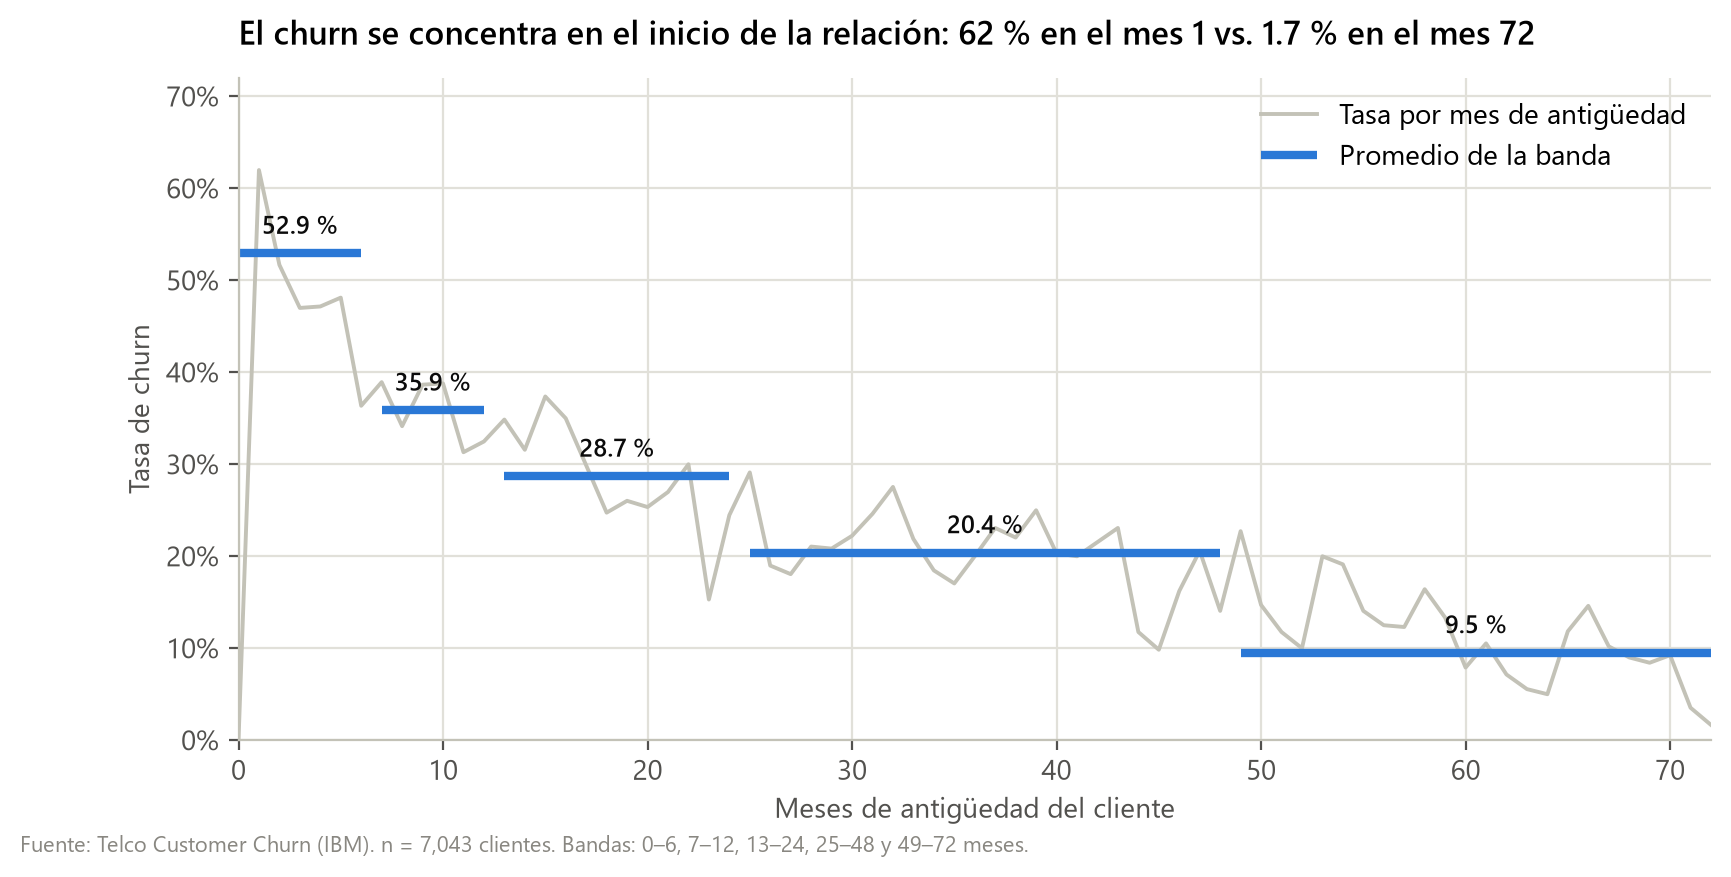
\includegraphics[width=0.83\textwidth]{f01_churn_ciclo_vida.png}
\caption{Churn por mes de antigüedad y promedio por banda. El primer mes concentra el mayor riesgo (62\,\%).}
\end{figure}
\begin{figure}[H]
\centering
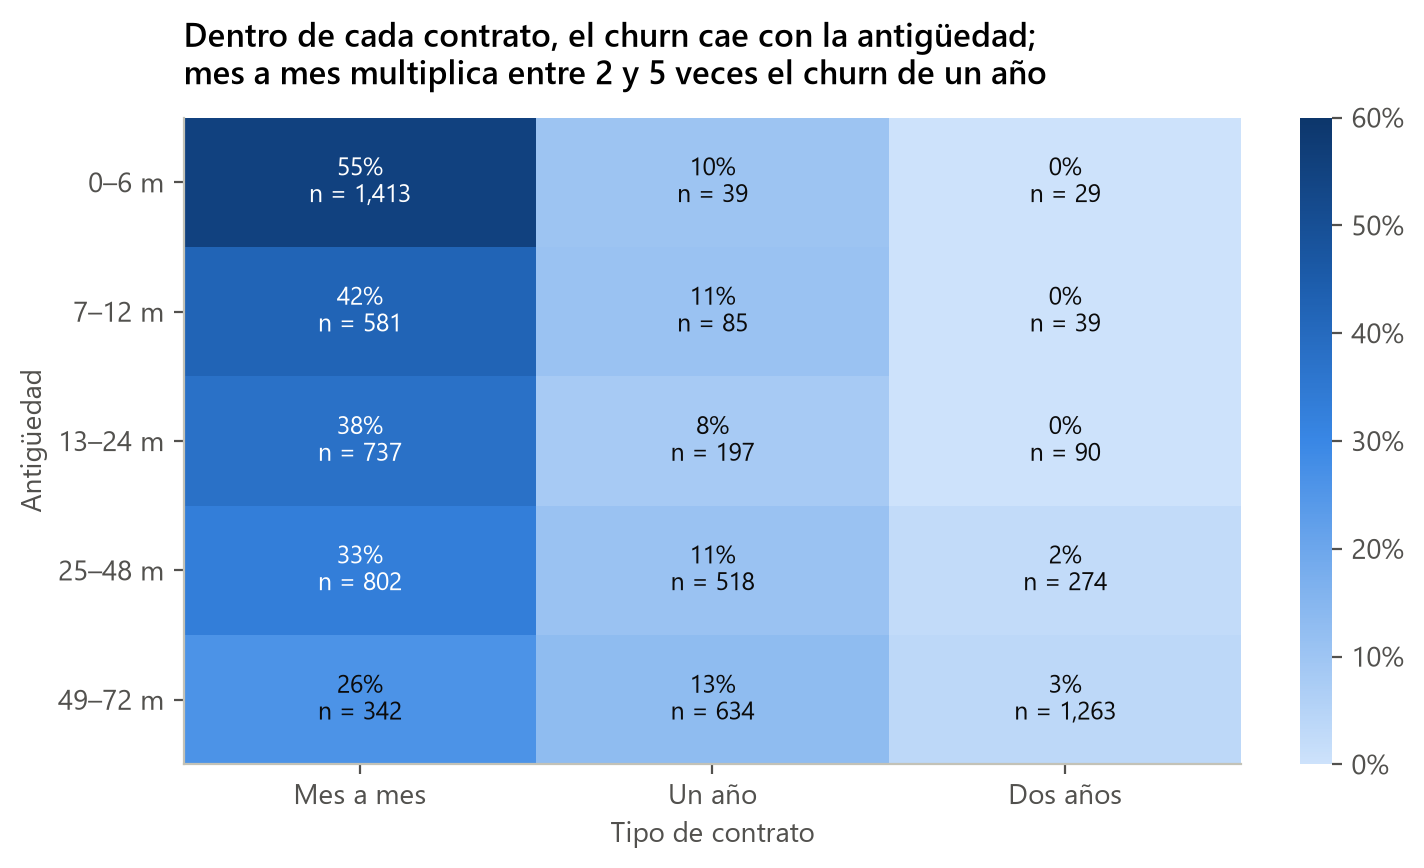
\includegraphics[width=0.62\textwidth]{f02_heatmap_contrato_antiguedad.png}
\caption{Churn por contrato y banda de antigüedad (cohortes por antigüedad, con el tamaño de cada celda).}
\end{figure}
\textbf{Qué muestra.} El churn cae de 52.9\,\% (0–6 meses) a 9.5\,\% (49–72 meses), y la caída ocurre \emph{dentro} de cada contrato: en mes a mes pasa de 55\,\% a 26\,\%. \textbf{Qué significa.} Los primeros meses son la ventana crítica, y no se trata solo de un efecto de mezcla de contratos. \textbf{Qué implica.} Un onboarding temprano (palanca L4) ataca la etapa de mayor riesgo. \emph{Limitación:} los clientes antiguos son sobrevivientes, así que la curva describe tasas condicionales y no la trayectoria de una cohorte de altas. \begin{figure}[H]
\centering
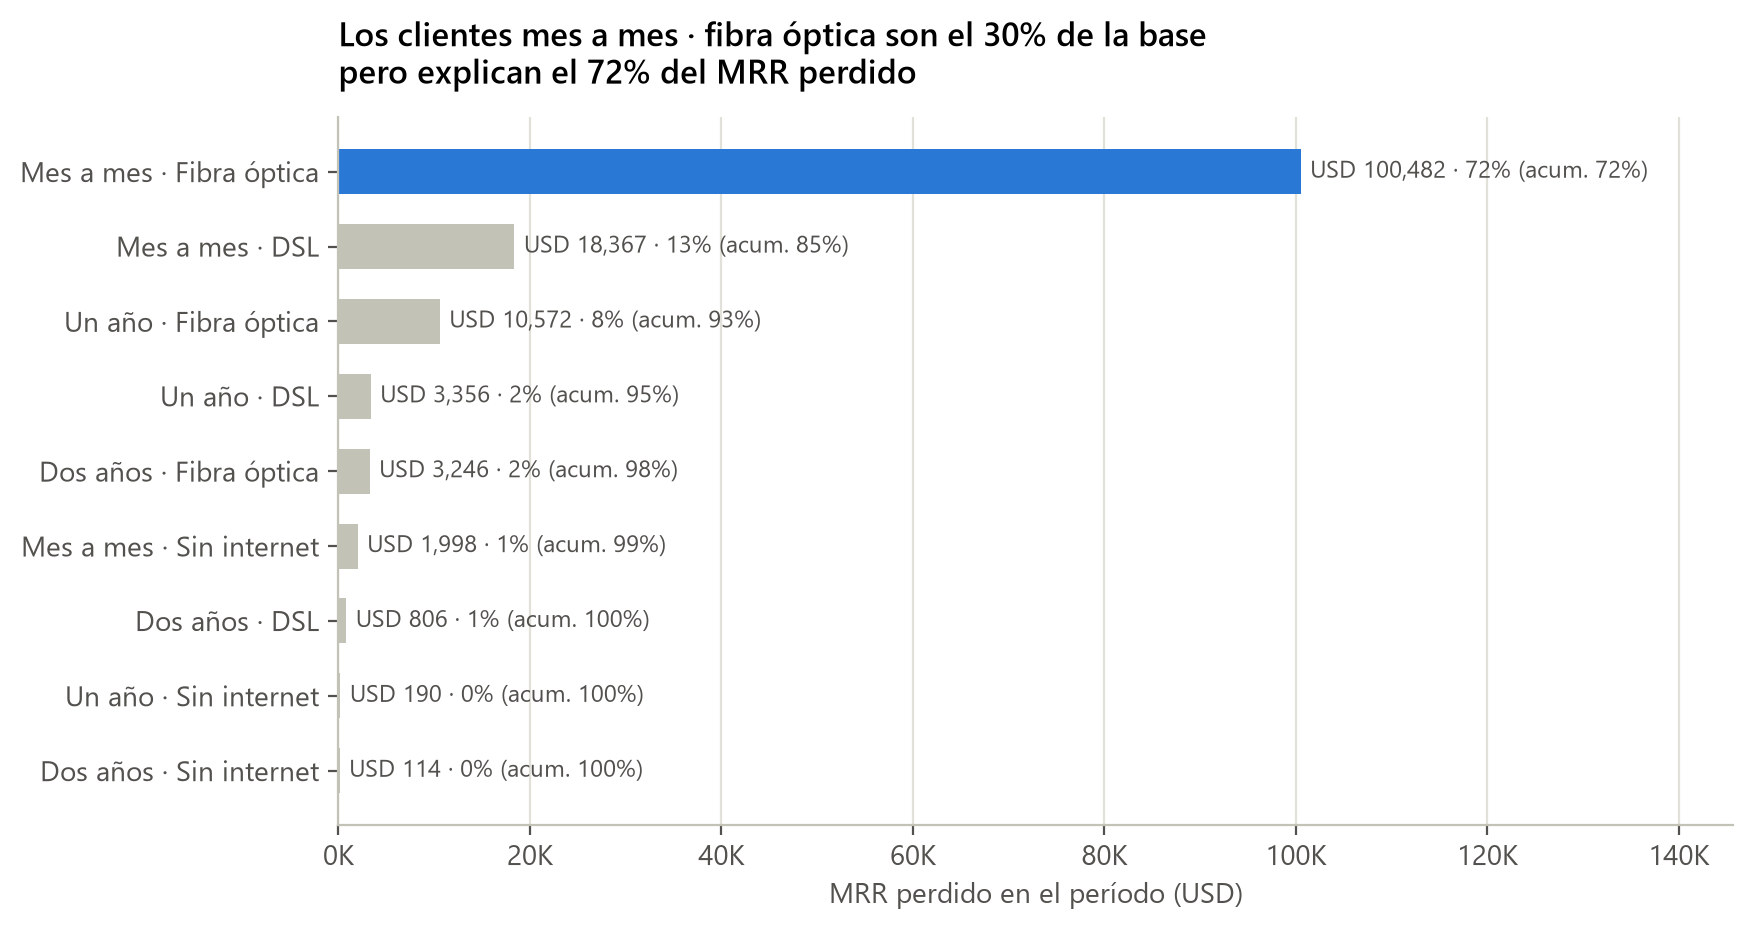
\includegraphics[width=0.7\textwidth]{f04_contribucion_mrr_perdido.png}
\caption{Contribución de cada segmento (contrato × internet) al MRR perdido.}
\end{figure}
En contribución, \textbf{mes a mes con fibra concentra el 72\,\% del MRR perdido con el 30\,\% de los clientes}, y mes a mes con DSL suma otro 13\,\%.

\subsection{Segmentación de desempeño y drivers ajustados}
\begin{figure}[H]
\centering
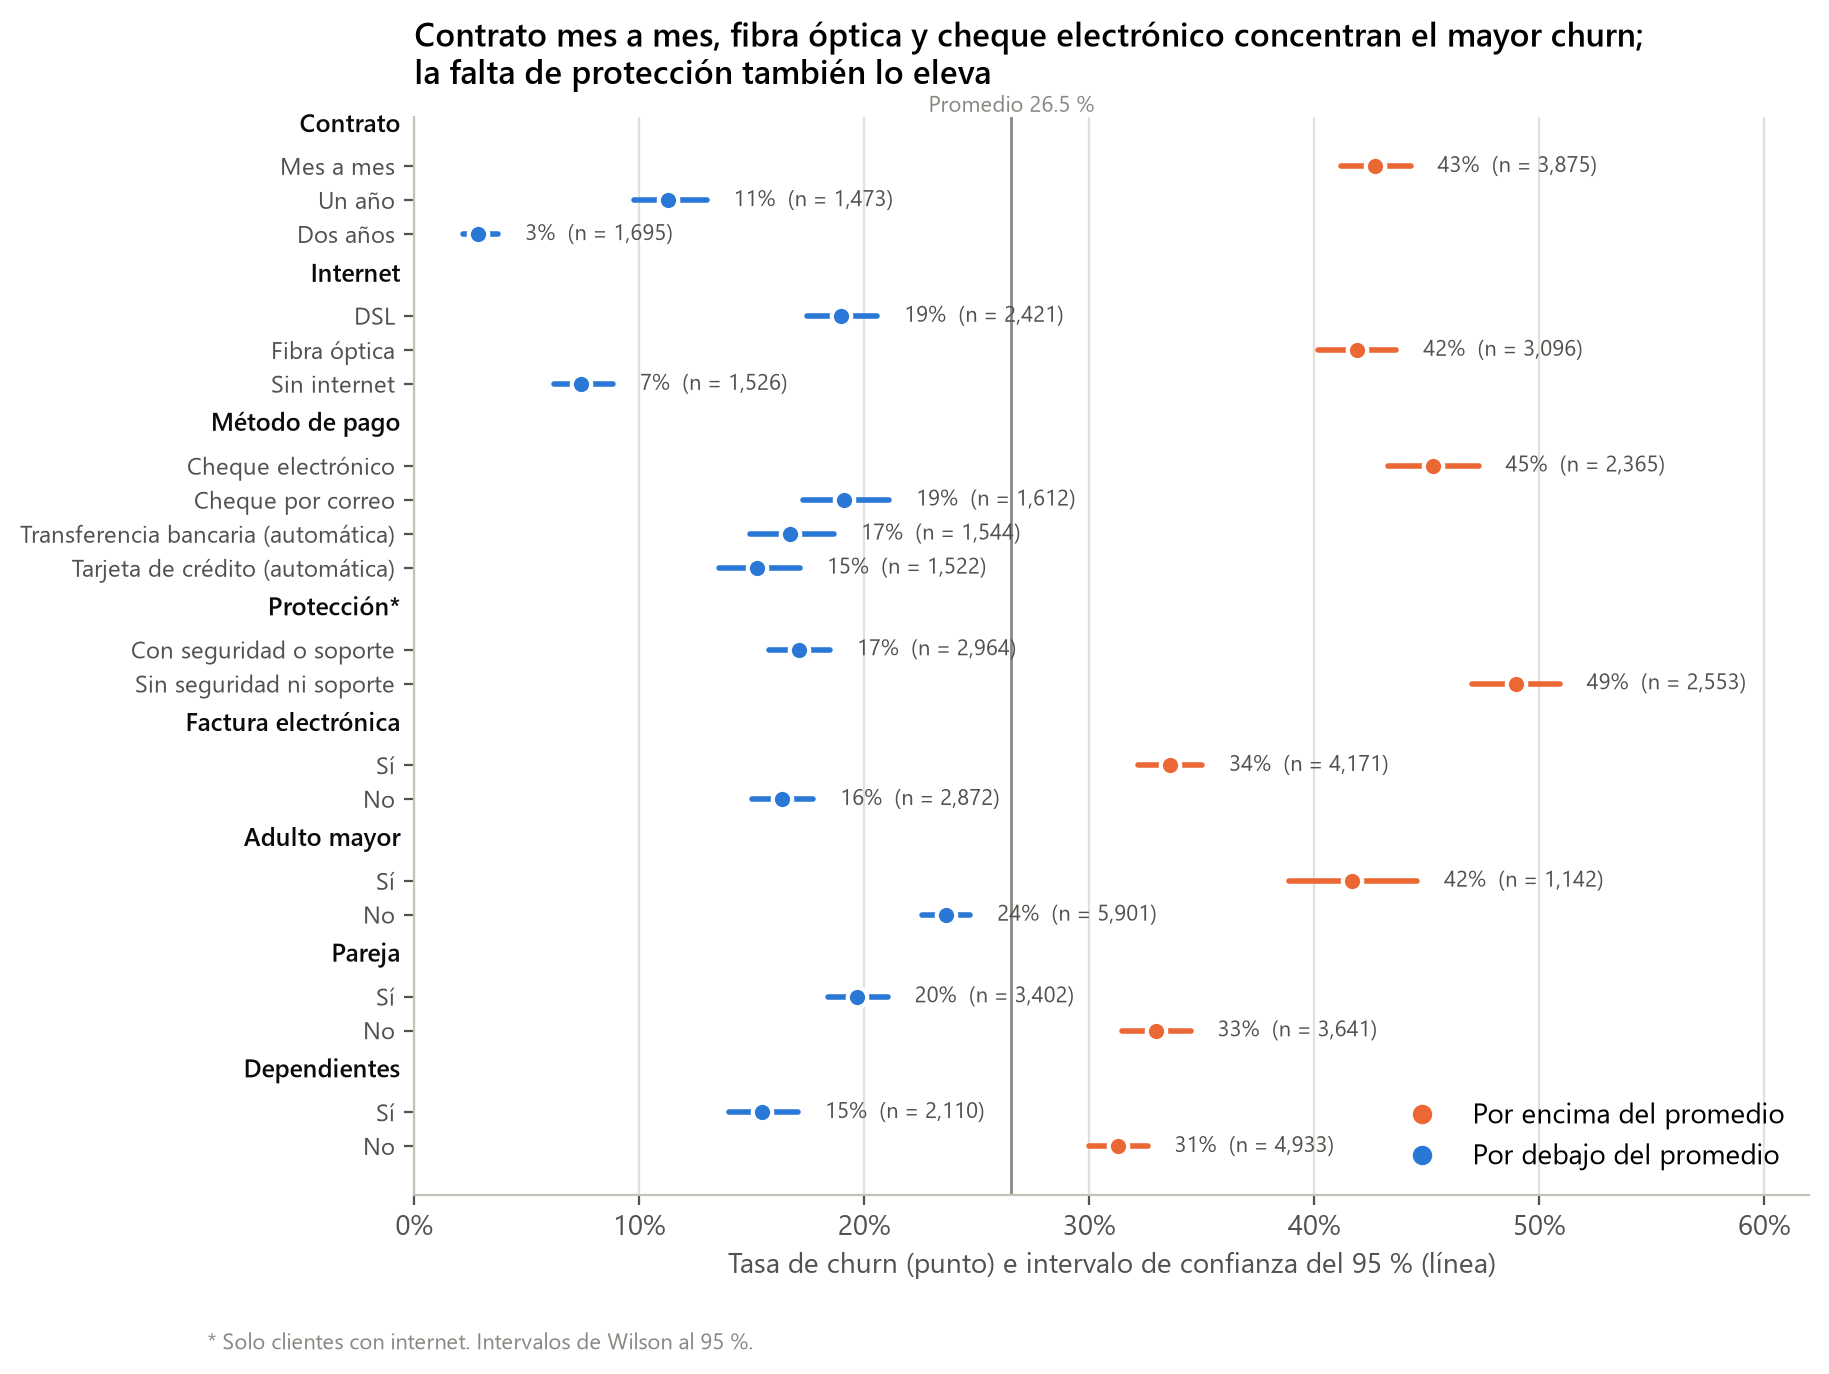
\includegraphics[width=0.74\textwidth]{f03_churn_por_segmento.png}
\caption{Churn por segmento con intervalos de confianza de Wilson al 95\,\%.}
\end{figure}
La segmentación bruta muestra tasas de 42.7\,\% en mes a mes, 41.9\,\% en fibra, 45.3\,\% con cheque electrónico y 49.0\,\% sin seguridad ni soporte. Todas tienen intervalos estrechos que no se solapan con el promedio. \begin{figure}[H]
\centering
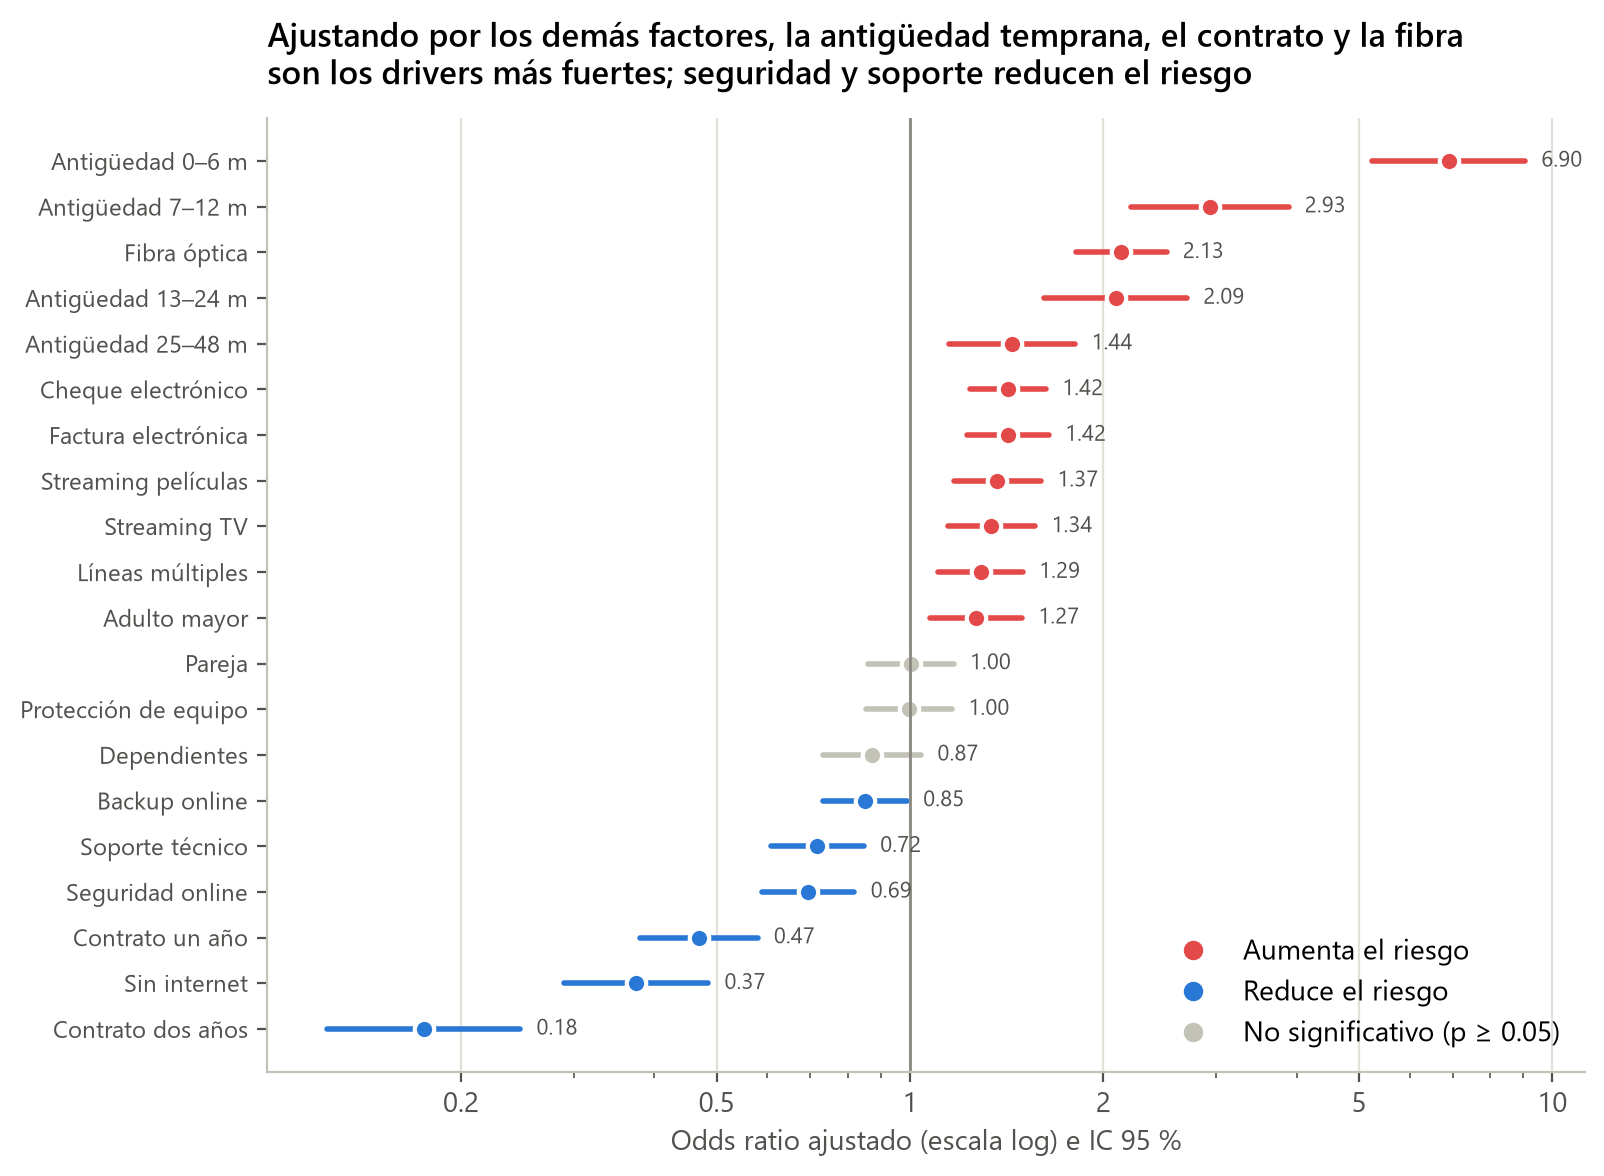
\includegraphics[width=0.66\textwidth]{f05_drivers_odds_ratio.png}
\caption{Odds ratios de una regresión logística (numpy, IRLS) que ajusta todos los factores a la vez, con IC 95\,\%.}
\end{figure}
El \textbf{modelo logístico} confirma que estas relaciones persisten al ajustar por los demás factores:
\begin{itemize}
  \item \textbf{Antigüedad 0–6 m}: OR 6.9 frente a 49–72 m.
  \item \textbf{Contrato}: dos años OR 0.18 y un año OR 0.47 frente a mes a mes.
  \item \textbf{Fibra}: OR 2.1.
  \item \textbf{Cheque electrónico y factura electrónica}: OR 1.4 cada uno.
  \item \textbf{Seguridad online} (OR 0.70) y \textbf{soporte técnico} (OR 0.72) reducen el riesgo.
\end{itemize}
Pareja y dependientes \emph{dejan de ser significativos} al ajustar: su efecto bruto se explicaba por contrato y antigüedad. La fibra mantiene un riesgo alto aun ajustada, lo que apunta a un problema de propuesta de valor (precio o calidad) que corresponde a la alternativa D y que estos datos no permiten diagnosticar.

\begin{table}[H]
\centering\footnotesize
\caption{Uplift descriptivo dentro de estratos homogéneos (diferencia de churn en puntos porcentuales, IC 95\,\%). Son asociaciones, no efectos causales.}
\begin{tabularx}{\textwidth}{@{}Xlrrrr@{}}
\toprule
Estrato · comparación & n (A / B) & Churn A & Churn B & Diferencia & IC 95\,\% \\
\midrule
Mes a mes + fibra · con vs. sin seguridad online & 354 / 1,774 & 37.0\,\% & 58.1\,\% & −21.1 pp & [−26.6, −15.6] \\
Mes a mes + fibra · con vs. sin soporte técnico & 332 / 1,796 & 38.9\,\% & 57.5\,\% & −18.7 pp & [−24.4, −12.9] \\
Mes a mes + fibra · pago automático vs. cheque electrónico & 620 / 1,307 & 43.7\,\% & 60.4\,\% & −16.7 pp & [−21.4, −11.9] \\
Nuevos (0–12 m) con internet · con vs. sin protección & 470 / 1,203 & 37.0\,\% & 64.1\,\% & −27.1 pp & [−32.2, −21.9] \\
Nuevos (0–12 m) · un año vs. mes a mes & 124 / 1,994 & 10.5\,\% & 51.4\,\% & −40.9 pp & [−46.7, −35.0] \\
\bottomrule
\end{tabularx}
\end{table}
Estas brechas \textbf{acotan} los supuestos de efecto de cada palanca (sección 10), que se descuentan fuertemente porque quienes eligen protección, pago automático o contrato anual pueden ser clientes distintos (sesgo de selección).

% ===========================================================================
\section{Medición de impacto, ROI y priorización}
% ===========================================================================
\subsection{Score de riesgo y matriz de priorización}
Con el mismo modelo logístico, cada cliente recibe una probabilidad de churn \textbf{fuera de muestra} (validación cruzada de 5 pliegues). El AUC es \textbf{0.85} y la calibración es buena por deciles (Anexo D). El score se usa para \emph{ordenar}, no como pronóstico exacto. Con él se definen tres niveles para los 5,174 clientes activos:
\begin{itemize}
  \item \textbf{Alto} (score $\geq$ 40\,\%): 820 clientes, USD 64 mil de MRR y \textbf{53\,\% del MRR en riesgo esperado} (USD 36.0 mil de 68.1 mil).
  \item \textbf{Medio} (20–40\,\%): 972 clientes y 28\,\% del MRR en riesgo.
  \item \textbf{Bajo}: 3,382 clientes y 19\,\% del MRR en riesgo.
\end{itemize}
\begin{figure}[H]
\centering
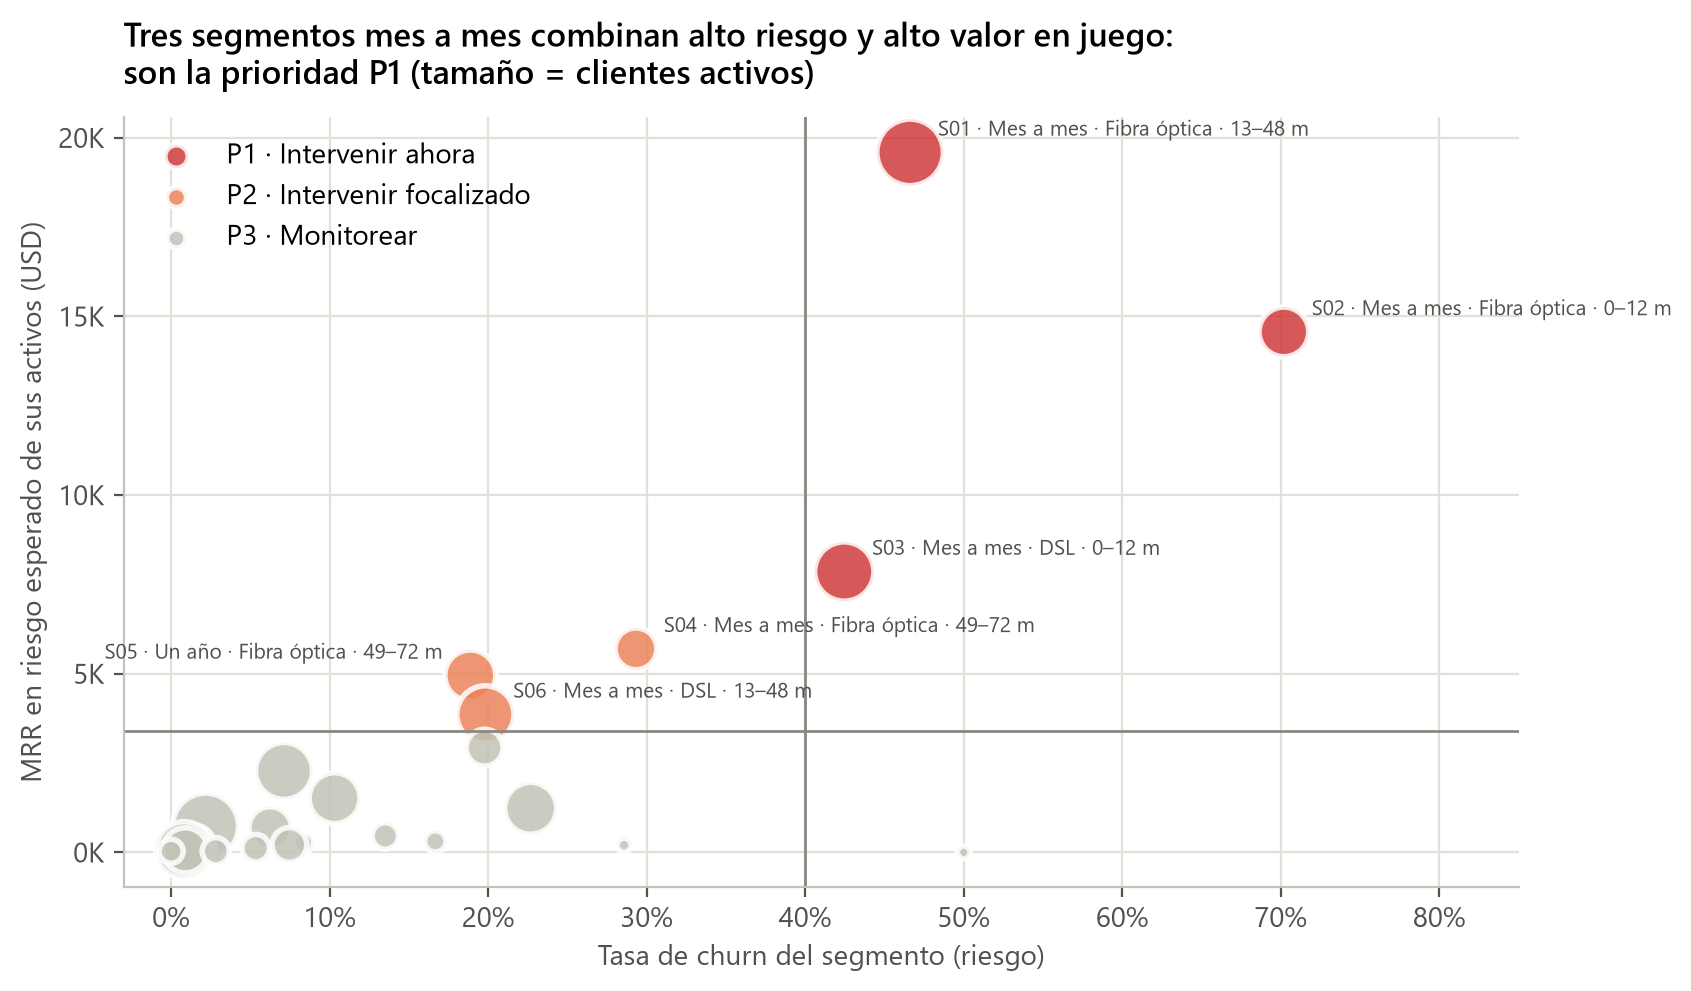
\includegraphics[width=0.74\textwidth]{f07_matriz_priorizacion.png}
\caption{Matriz de priorización de segmentos (contrato × internet × etapa). P1: churn $\geq$ 40\,\% y $\geq$ 5\,\% del MRR en riesgo (con al menos 30 clientes).}
\end{figure}
Los tres segmentos \textbf{P1} son \emph{mes a mes · fibra · 13–48 m} (505 activos, churn 46.6\,\%, USD 19.6 mil en riesgo), \emph{mes a mes · fibra · 0–12 m} (273, 70.2\,\%, USD 14.6 mil) y \emph{mes a mes · DSL · 0–12 m} (397, 42.5\,\%, USD 7.9 mil). Juntos suman el 62\,\% del MRR en riesgo esperado.

\subsection{Palancas, supuestos y escenarios}
Cada cliente activo recibe una \textbf{palanca principal}, ordenada por costo: primero L4 onboarding temprano (antigüedad $\leq$ 6 m), luego L2 bundle de protección (fibra sin seguridad ni soporte), luego L3 pago automático (cheque electrónico) y al final L1 migración a contrato anual (mes a mes), porque presiona el ARPU. El valor esperado por cliente es $p_{\text{churn}} \times \text{aceptación} \times \text{reducción atribuible} \times \text{cargo} \times \text{margen} \times \text{horizonte}$. El costo es contacto + aceptación × incentivo.

\begin{table}[H]
\centering\footnotesize
\caption{Supuestos explícitos por palanca y escenario (conservador / base / optimista).}
\begin{tabularx}{\textwidth}{@{}lXccc@{}}
\toprule
Palanca & Incentivo y costo & Aceptación & Reducción atribuible & Evidencia que la acota \\
\midrule
L4 Onboarding temprano & Acompañamiento en los meses 1–3; USD 8 por cliente contactado & 50 / 65 / 80\,\% & 5 / 10 / 20\,\% & Churn 0–6 m de 52.9\,\% \\
L2 Bundle de protección & 3 meses sin costo de seguridad + soporte (lista USD 10.05/mes; costo variable) & 20 / 30 / 40\,\% & 10 / 20 / 30\,\% & −21 pp observacional \\
L3 Pago automático & Crédito único de USD 10 & 20 / 30 / 40\,\% & 10 / 15 / 25\,\% & OR 1.42; −17 pp \\
L1 Migración anual & 10\,\% de descuento por 12 meses (1.2 × cargo) & 15 / 25 / 35\,\% & 20 / 35 / 50\,\% & −41 pp, con fuerte autoselección \\
\midrule
\multicolumn{5}{@{}l}{Margen de contribución 45 / 55 / 65\,\%; horizonte de permanencia del cliente salvado 6 / 12 / 18 meses; contacto USD 2 (L1–L3).} \\
\bottomrule
\end{tabularx}
\end{table}

\begin{table}[H]
\centering\footnotesize
\caption{ROI estimado por alternativa y escenario.}
\begin{tabular}{@{}lrrrrrr@{}}
\toprule
Alternativa & Clientes & ROI cons. & ROI base & ROI opt. & Costo base & Contribución base \\
\midrule
B · Descuento masivo (L1 a todo mes a mes) & 2,220 & −85\,\% & \textbf{−32\,\%} & +77\,\% & USD 45,374 & USD 30,889 \\
C · Programa sin focalizar (todas las palancas) & 2,839 & −79\,\% & +0\,\% & +205\,\% & USD 24,997 & USD 25,079 \\
C · Programa focalizado (riesgo alto) & 820 & −48\,\% & \textbf{+179\,\%} & +839\,\% & USD 5,191 & USD 14,482 \\
\bottomrule
\end{tabular}
\end{table}

\begin{figure}[H]
\centering
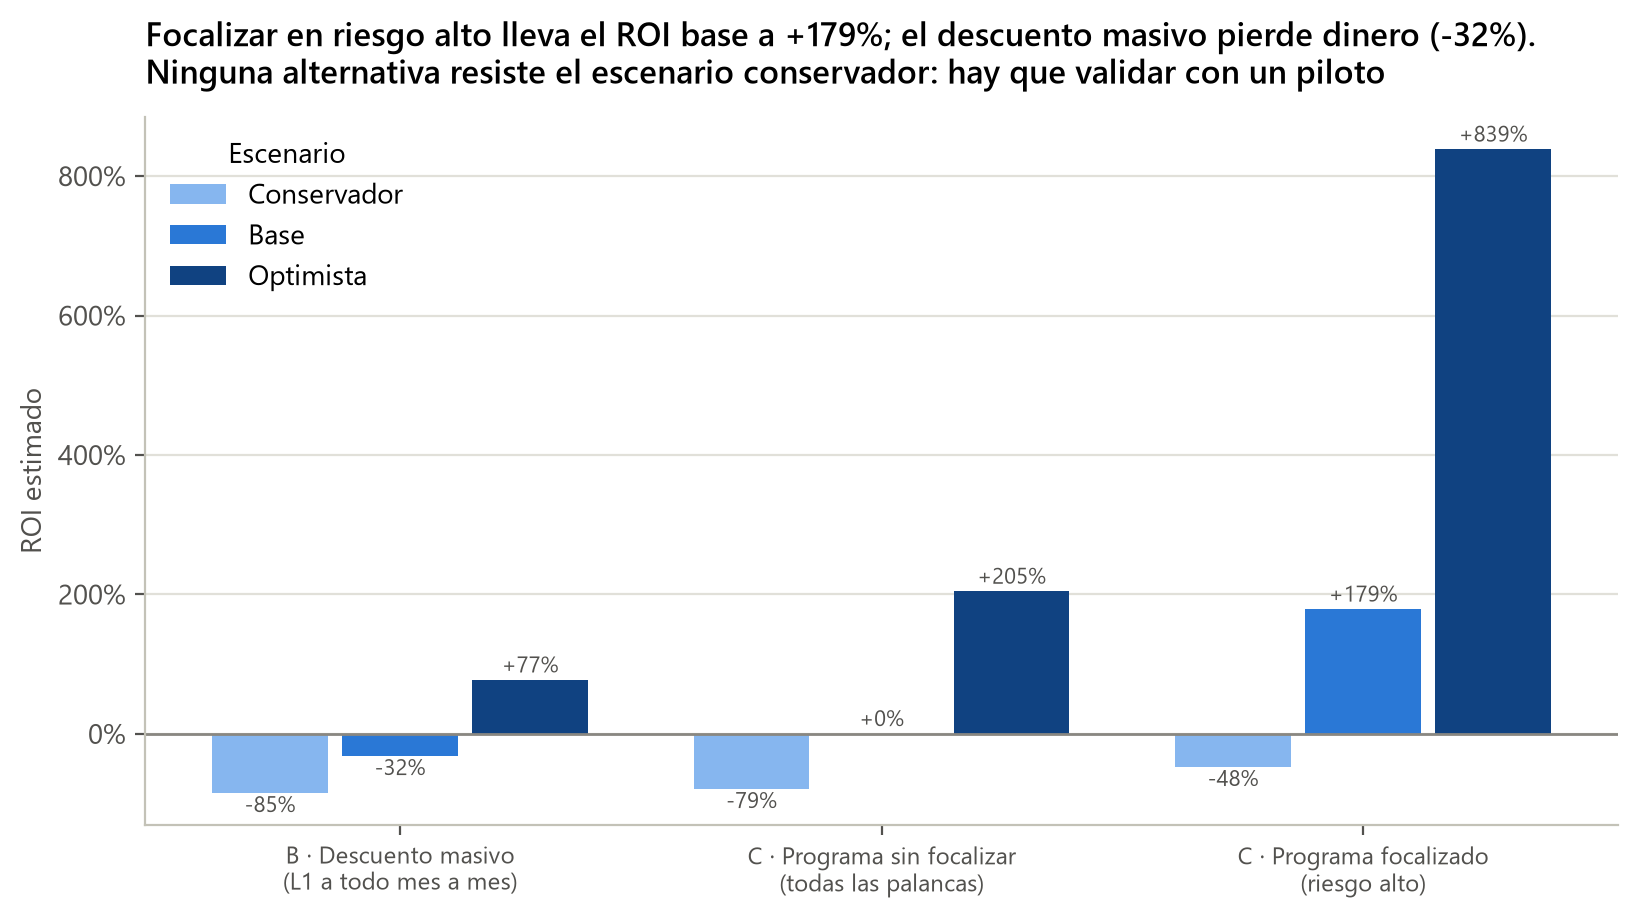
\includegraphics[width=0.7\textwidth]{f08_roi_alternativas.png}
\caption{ROI estimado por alternativa y escenario.}
\end{figure}
\begin{figure}[H]
\centering
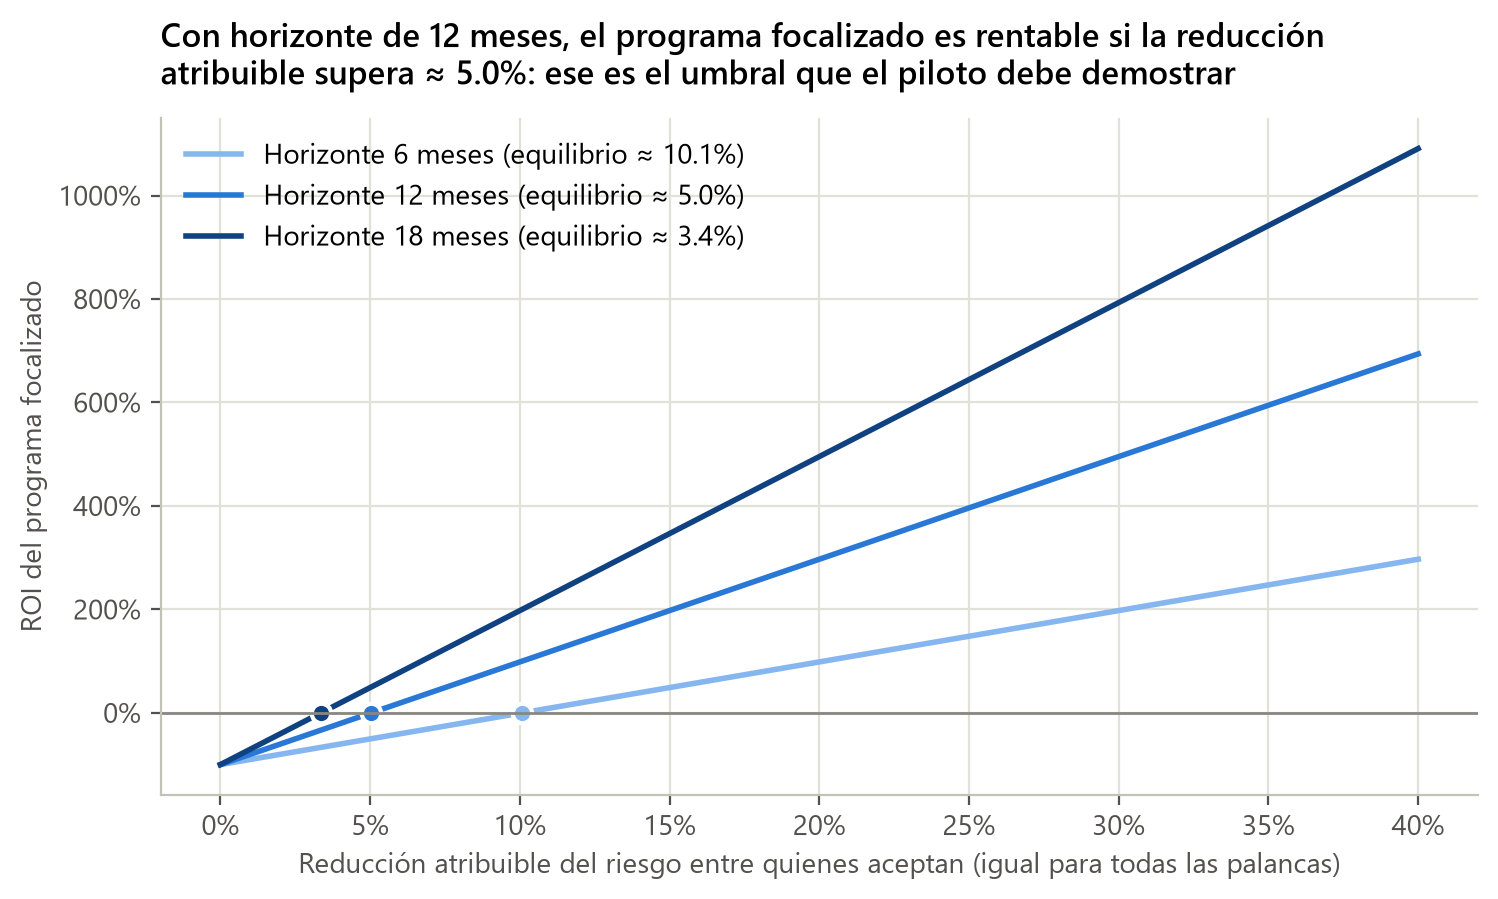
\includegraphics[width=0.64\textwidth]{f09_sensibilidad_roi.png}
\caption{Sensibilidad del ROI del programa focalizado a la reducción atribuible y al horizonte.}
\end{figure}
\textbf{Lectura.}
\begin{itemize}
  \item \textbf{Focalizar multiplica el retorno.} El programa focalizado salva unos 28 clientes por corte (USD 2,194 de MRR al mes) a un costo de USD 184 por cliente salvado. El descuento masivo cuesta USD 677 por cliente salvado.
  \item \textbf{Por palanca}, en el escenario base y en riesgo alto, el ROI es de +236\,\% para L4, +208\,\% para L2, +160\,\% para L3 y −18\,\% para L1.
  \item \textbf{Regla de decisión (Sesión 5).} Ninguna alternativa resiste el escenario conservador, así que la recomendación es \textbf{prudente}: piloto antes de escalar. El análisis de sensibilidad da el criterio de escalamiento: con 12 meses de horizonte, el programa es rentable si la reducción atribuible supera ≈ 5\,\% (10\,\% con 6 meses).
\end{itemize}

\subsection{Diseño del piloto A/B (Sesión 6)}
\begin{table}[H]
\centering\footnotesize
\caption{Diseño experimental del piloto.}
\begin{tabularx}{\textwidth}{@{}>{\bfseries}P{3.4cm}X@{}}
\toprule
Hipótesis & Asignar a cada cliente de riesgo alto su palanca reduce el churn a 90 días frente a no intervenir. \\
Población y aleatorización & Clientes activos con score $\geq$ 40\,\% y palanca distinta de L0, asignados 50/50 a nivel cliente y estratificados por palanca. \\
Métricas & Primaria: churn a 90 días. Secundarias: aceptación, adopción de protección, cambio a pago automático. Guardrails: ARPU, costo por salvado, reclamos. \\
Poder & 820 elegibles por corte (410 por brazo). Churn esperado en el control: 55.9\,\%. El MDE con un corte es de 9.7 pp y el efecto esperado en el escenario base es de 3.4 pp, así que se necesitan unos 3,305 clientes por brazo, es decir, \textbf{acumular cohortes mensuales} (≈ 9 con esta muestra; menos en la base real de la operadora). \\
Controles & Sample Ratio Mismatch, hipótesis registrada antes de ver resultados, sin detención temprana, separación de uplift absoluto (pp) y relativo. \\
\bottomrule
\end{tabularx}
\end{table}

% ===========================================================================
\section{Diseño del dashboard y justificación de páginas}
% ===========================================================================
El dashboard está construido en \textbf{Power BI} como proyecto PBIP (\texttt{powerbi/DataForge\_Telco\_Churn.pbip}), con un modelo semántico en TMDL y un reporte en PBIR, versionables en Git.
\begin{itemize}
  \item \textbf{Modelo.} Es un esquema estrella: \texttt{fact\_clientes} (granularidad cliente-corte) se relaciona con siete dimensiones (antigüedad, contrato, internet, pago, riesgo, palanca, segmento) mediante relaciones uno a muchos con filtro simple. Seis tablas desconectadas alimentan el simulador y las definiciones.
  \item \textbf{Medidas.} Son \textbf{39 medidas DAX} en la tabla \texttt{Medidas}, organizadas en carpetas (base, estratégicos, operativos, diagnóstico y balance, alertas, simulador). Usan \texttt{DISTINCTCOUNT}, \texttt{DIVIDE}, \texttt{CALCULATE}, \texttt{SWITCH(TRUE())}, \texttt{SUMX} y \texttt{LOOKUPVALUE} (Anexo B).
  \item \textbf{Reconciliación.} Las cifras cuadran con el notebook: NSM 69.5\,\%, ROI focalizado +179\,\%, MRR en riesgo USD 68 mil.
\end{itemize}

\begin{table}[H]
\centering\footnotesize
\caption{Páginas del dashboard: audiencia, pregunta y acción.}
\begin{tabularx}{\textwidth}{@{}P{2.3cm}P{2.4cm}XX@{}}
\toprule
Página & Audiencia & Pregunta y visuales & Decisión o acción \\
\midrule
1 · Resumen ejecutivo & Comité y Gerencia & ¿Cuánto MRR perdemos y dónde? 6 KPIs con semáforo (NSM, MRR perdido, churn, churn temprano, \% a plazo, ARPU), línea de churn por mes de vida (temporal), barras por contrato e internet, 4 filtros y lectura ejecutiva. & Dimensionar el problema y fijar el foco del mes. \\
2 · Diagnóstico & Gerencia y Analítica & ¿Por qué abandonan? Matriz antigüedad × contrato (heatmap), churn por pago y por protección, odds ratios y dispersión de segmentos ARPU × churn. Interacción cruzada entre visuales. & Elegir la palanca según el driver. \\
3 · Monitoreo y acción & Gerencia de Retención & ¿A quién intervenir y con qué retorno? Clientes y MRR de riesgo alto, MRR en riesgo esperado, ROI focalizado vs. sin focalizar con segmentador de escenario, tabla de priorización P1–P3 con palanca y responsable, regla de decisión y plan de monitoreo con umbrales. & Asignar la lista de trabajo y el presupuesto; activar alertas. \\
4 · Definiciones & Todos & Diccionario de métricas, supuestos por escenario y notas de interpretación. & Leer las métricas sin ambigüedad. \\
\bottomrule
\end{tabularx}
\end{table}

\begin{figure}[H]
\centering
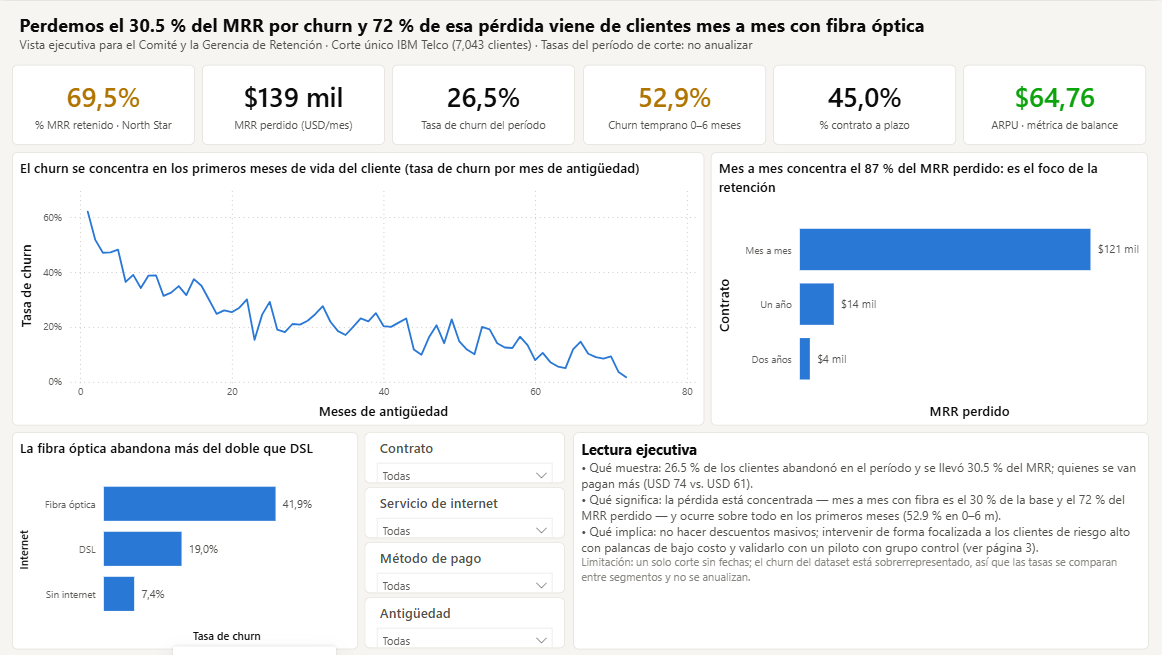
\includegraphics[width=0.92\textwidth]{dashboard_p1.png}
\caption{Página 1 · Resumen ejecutivo (captura de Power BI Desktop con datos). Los KPIs usan color de semáforo; los títulos son interpretativos.}
\end{figure}
\begin{figure}[H]
\centering
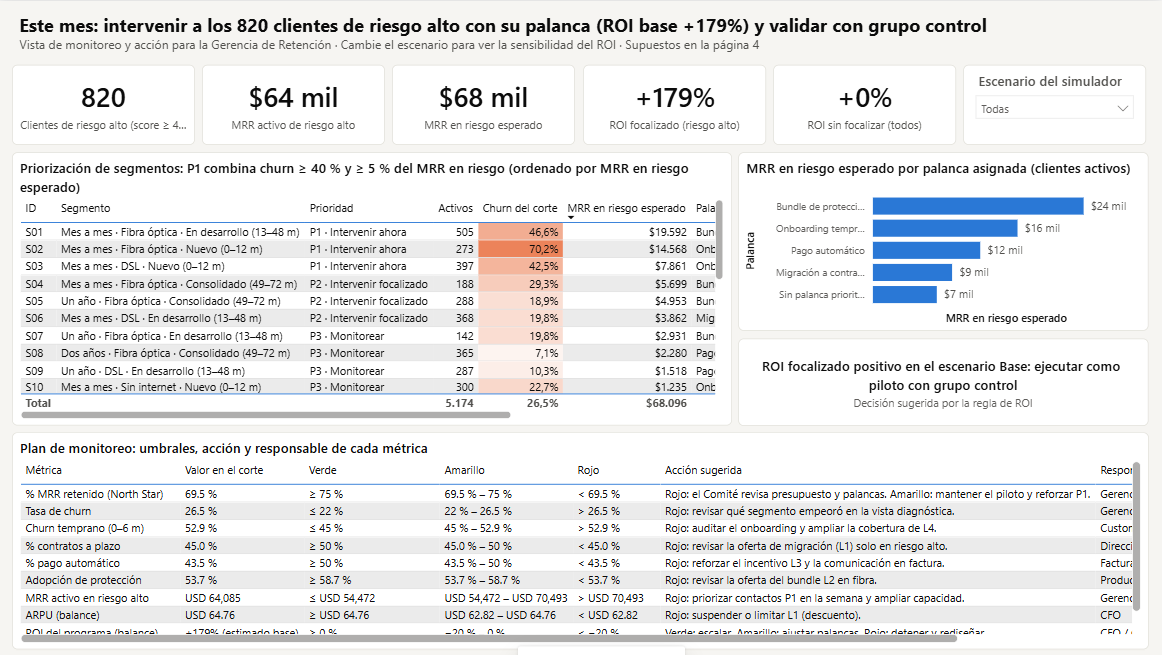
\includegraphics[width=0.92\textwidth]{dashboard_p3.png}
\caption{Página 3 · Monitoreo y acción: priorización de segmentos, simulador de ROI por escenario, regla de decisión y plan de monitoreo.}
\end{figure}
\textbf{Requisitos del enunciado.} Las tres páginas mínimas (más una de definiciones), 9 métricas relevantes en las vistas ejecutiva y de acción, filtros por contrato, internet, pago, antigüedad y escenario, una visualización temporal (ciclo de vida), visualizaciones de segmentación y contribución, y lógica de alerta (semáforos y prioridad P1–P3). En el diseño, cada página tiene un titular interpretativo, una paleta consistente con el notebook y la exploración separada de la comunicación ejecutiva. Las capturas de las páginas 2 y 4 están en el Anexo C.

% ===========================================================================
\section{Plan de monitoreo y acciones sugeridas}
% ===========================================================================
\begin{table}[H]
\centering\footnotesize
\caption{Plan de monitoreo y acción (Plantilla 4). Umbrales verde / amarillo / rojo definidos sobre el corte inicial.}
\begin{tabularx}{\textwidth}{@{}P{2.8cm}P{1.6cm}P{3.6cm}XP{1.7cm}@{}}
\toprule
Métrica & Corte & Umbral (verde · amarillo · rojo) & Acción sugerida & Responsable \\
\midrule
\% MRR retenido (NSM) & 69.5\,\% & $\geq$ 75 · 69.5–75 · $<$ 69.5\,\% & Rojo: el Comité revisa presupuesto y palancas. Amarillo: mantener el piloto y reforzar P1. & Gerencia Retención \\
Tasa de churn & 26.5\,\% & $\leq$ 22 · 22–26.5 · $>$ 26.5\,\% & Revisar qué segmento empeoró en la página 2. & Gerencia Retención \\
Churn temprano 0–6 m & 52.9\,\% & $\leq$ 45 · 45–52.9 · $>$ 52.9\,\% & Auditar el onboarding y ampliar la cobertura de L4. & Customer Success \\
\% contrato a plazo & 45.0\,\% & $\geq$ 50 · 45–50 · $<$ 45\,\% & Revisar la oferta L1, solo en riesgo alto. & Dir. Comercial \\
\% pago automático & 43.5\,\% & $\geq$ 50 · 43.5–50 · $<$ 43.5\,\% & Reforzar el incentivo L3 y la comunicación en factura. & Facturación \\
Adopción de protección & 53.7\,\% & $\geq$ 58.7 · 53.7–58.7 · $<$ 53.7\,\% & Revisar la oferta del bundle L2 en fibra. & Producto \\
MRR activo en riesgo alto & USD 64,085 & $\leq$ 54,472 · hasta 70,493 · $>$ 70,493 & Priorizar los contactos P1 en la semana y ampliar capacidad. & Gerencia Retención \\
ARPU (balance) & USD 64.76 & $\geq$ 64.76 · 62.82–64.76 · $<$ 62.82 & Suspender o limitar el descuento L1. & CFO \\
ROI del programa & +179\,\% (est.) & $\geq$ 0 · −20–0 · $<$ −20\,\% & Verde: escalar. Amarillo: ajustar palancas. Rojo: detener y rediseñar. & CFO \\
Uplift del piloto (90 d) & Sin medir & Significativo y $\geq$ equilibrio · positivo n.s. · nulo & Verde: escalar a toda la población elegible. & Analítica \\
\bottomrule
\end{tabularx}
\end{table}

% ===========================================================================
\section{Recomendación ejecutiva}
% ===========================================================================
\begin{caja}
\textbf{Decisión recomendada.} Aprobar un \textbf{piloto del programa focalizado de retención} sobre los clientes activos de riesgo alto (820 en este corte) con grupo control 50/50, empezando por las palancas de bajo costo: onboarding temprano (L4), bundle de protección (L2) y pago automático (L3). La migración con descuento (L1) queda limitada a los casos residuales de riesgo alto. \textbf{No} aprobar descuentos masivos a los clientes mes a mes.
\end{caja}
\textbf{Evidencia que la soporta.}
\begin{itemize}
  \item La pérdida está concentrada: 72\,\% del MRR perdido en mes a mes con fibra, y 53\,\% del MRR en riesgo en el 16\,\% de los activos.
  \item Los drivers ajustados coinciden con las palancas: contrato, primeros meses, protección y pago.
  \item El ROI base del programa focalizado es de +179\,\%, frente a −32\,\% del descuento masivo.
  \item El umbral de equilibrio es bajo (≈ 5\,\% de reducción atribuible a 12 meses), así que el piloto tiene una meta alcanzable y verificable.
\end{itemize}
\textbf{Condiciones para escalar.} El uplift a 90 días debe ser significativo y superior al umbral de equilibrio, el ARPU no debe caer más de 3\,\% y el costo por cliente salvado debe quedar por debajo de USD 200. \textbf{Primeros 90 días:} mes 1, preparar la lista P1 y la aleatorización; meses 1 a 3, ejecutar las palancas y monitorear semanalmente las métricas líderes; mes 3, lectura del piloto y decisión de escalar con el Comité.

% ===========================================================================
\section{Limitaciones, riesgos y próximos pasos}
% ===========================================================================
\begin{itemize}
  \item \textbf{Datos.} Hay un único corte sin fecha calendario: no hay tendencia mensual ni estacionalidad. El churn está sobrerrepresentado y la ventana es ambigua, por lo que los montos son del período de corte y no se anualizan. El dataset es sintético.
  \item \textbf{Causalidad.} Las brechas por protección, pago y contrato son observacionales y pueden reflejar autoselección. El modelo describe asociaciones ajustadas, no efectos de intervención.
  \item \textbf{Supuestos económicos.} El margen, el horizonte, los costos y la aceptación son supuestos. El escenario conservador es negativo, así que la recomendación depende del piloto.
  \item \textbf{Riesgo de incentivos.} Optimizar el \% de contratos a plazo o la tasa de churn puede destruir ARPU (Goodhart). Por eso se monitorean el ARPU y el ROI como balance.
  \item \textbf{Próximos pasos.} (1) Cargar cortes mensuales con \texttt{fecha\_corte} y fecha de alta para tener tendencia y cohortes de adquisición reales. (2) Integrar el CRM de campañas y los costos reales. (3) Ejecutar el piloto A/B. (4) Investigar la propuesta de valor de la fibra (alternativa D) con datos de calidad de servicio, tickets y precios de la competencia. (5) Recalibrar el score con cada corte.
\end{itemize}

% ===========================================================================
\section*{Referencias}
% ===========================================================================
{\footnotesize
\begin{itemize}[leftmargin=1em]
  \item IBM. \emph{Telco Customer Churn} (IBM Sample Data Sets). Publicado en Kaggle por blastchar: \url{https://www.kaggle.com/datasets/blastchar/telco-customer-churn}.
  \item De Mier Medellín, J. (2026). Material de clase, sesiones 1 a 8, \emph{Decision Intelligence \& Business Analytics}. Escuela Colombiana de Ingeniería Julio Garavito.
  \item Provost, F. y Fawcett, T. (2013). \emph{Data Science for Business}. O'Reilly.
  \item Croll, A. y Yoskovitz, B. (2013). \emph{Lean Analytics}. O'Reilly.
  \item Knaflic, C. N. (2015). \emph{Storytelling with Data}. Wiley. · Few, S. (2013). \emph{Information Dashboard Design}. Analytics Press.
  \item Kohavi, R., Tang, D. y Xu, Y. (2020). \emph{Trustworthy Online Controlled Experiments}. Cambridge University Press.
  \item Gertler, P. et al. (2016). \emph{Impact Evaluation in Practice}. Banco Mundial.
  \item Kimball Group. \emph{Dimensional Modeling Techniques}. · Microsoft Learn. \emph{Understand star schema and the importance for Power BI}.
\end{itemize}}

% ===========================================================================
% ANEXOS
% ===========================================================================
\clearpage
\appendix
\renewcommand{\thesection}{\Alph{section}}
\section{Diccionario técnico de métricas}
Generado automáticamente desde \texttt{powerbi/data/dim\_metricas.csv}, la misma fuente que la página 4 del dashboard.
\subsection*{A.1 \% MRR retenido (North Star)}
\begin{footnotesize}
\begin{longtable}{@{}p{0.27\textwidth}p{0.69\textwidth}@{}}
\toprule
\textbf{Tipo} & Tasa / North Star Metric \\
\textbf{Objetivo asociado} & Proteger el ingreso recurrente \\
\textbf{Decisión que soporta} & Cuánto presupuesto asignar a retención y si el programa funciona \\
\textbf{Definición de negocio} & Proporción del ingreso recurrente mensual que se conserva al cierre del período \\
\textbf{Fórmula} & 1 − Σ cargo\_mensual[churn = 1] / Σ cargo\_mensual \\
\textbf{Numerador} & MRR de clientes que abandonan en el período \\
\textbf{Denominador} & MRR de todos los clientes al inicio del período \\
\textbf{Unidad} & \% \\
\textbf{Ventana temporal} & Período de corte (mensual a futuro) \\
\textbf{Filtros de inclusión} & registro\_valido = 1 \\
\textbf{Exclusiones} & Ninguna en el corte; a futuro, cuentas internas y de prueba \\
\textbf{Dimensiones de segmentación} & Contrato, servicio de internet, método de pago, antigüedad, riesgo, palanca \\
\textbf{Meta o umbral} & ≥ 75 \% (verde); 69.5–75 \% (amarillo); < 69.5 \% (rojo) \\
\textbf{Dirección deseada} & Subir \\
\textbf{Métricas de balance} & ARPU, costo de retención, ROI del programa \\
\textbf{Dueño} & Gerencia de Retención \\
\textbf{Riesgos de interpretación} & Puede subir por alzas de precio a clientes que se quedan; con un solo corte no hay tendencia; la ventana del churn es ambigua \\
\textbf{Acción asociada} & Si cae al rojo, el Comité revisa el presupuesto y las palancas del mes \\
\textbf{Medida DAX} & [\% MRR Retenido] \\
\textbf{Valor en el corte} & 69.5 \% \\
\textbf{Fuente de datos} & df\_analitico (derivada de WA\_Fn-UseC\_-Telco-Customer-Churn.csv) / fact\_clientes en Power BI \\
\textbf{Frecuencia de actualización} & Mensual, con cada corte de clientes (hoy existe un solo corte) \\
\textbf{Granularidad} & Cliente (cálculo) → segmento y mes (reporte) \\
\textbf{Unidad de análisis} & Cliente \\
\bottomrule
\end{longtable}
\end{footnotesize}

\subsection*{A.2 Tasa de churn de clientes}
\begin{footnotesize}
\begin{longtable}{@{}p{0.27\textwidth}p{0.69\textwidth}@{}}
\toprule
\textbf{Tipo} & Tasa \\
\textbf{Objetivo asociado} & Retener clientes \\
\textbf{Decisión que soporta} & Qué segmentos intervenir \\
\textbf{Definición de negocio} & Porcentaje de clientes que abandonan en el período \\
\textbf{Fórmula} & DISTINCTCOUNT(customer\_id)[churn = 1] / DISTINCTCOUNT(customer\_id) \\
\textbf{Numerador} & Clientes únicos con churn = 1 \\
\textbf{Denominador} & Clientes únicos en el corte \\
\textbf{Unidad} & \% \\
\textbf{Ventana temporal} & Período de corte \\
\textbf{Filtros de inclusión} & registro\_valido = 1 \\
\textbf{Exclusiones} & Ninguna \\
\textbf{Dimensiones de segmentación} & Contrato, internet, pago, antigüedad, protección, demografía \\
\textbf{Meta o umbral} & ≤ 22 \% (verde); 22–26.5 \% (amarillo); > 26.5 \% (rojo) \\
\textbf{Dirección deseada} & Bajar \\
\textbf{Métricas de balance} & \% MRR retenido (pondera valor), ARPU \\
\textbf{Dueño} & Gerencia de Retención \\
\textbf{Riesgos de interpretación} & No pondera el valor del cliente; el corte sobrerrepresenta el churn (no anualizar); promediar tasas de segmentos sin ponderar la sesga \\
\textbf{Acción asociada} & Si un segmento supera el 40 \%, entra a la priorización P1/P2 \\
\textbf{Medida DAX} & [Tasa Churn] \\
\textbf{Valor en el corte} & 26.5 \% \\
\textbf{Fuente de datos} & df\_analitico (derivada de WA\_Fn-UseC\_-Telco-Customer-Churn.csv) / fact\_clientes en Power BI \\
\textbf{Frecuencia de actualización} & Mensual, con cada corte de clientes (hoy existe un solo corte) \\
\textbf{Granularidad} & Cliente (cálculo) → segmento y mes (reporte) \\
\textbf{Unidad de análisis} & Cliente \\
\bottomrule
\end{longtable}
\end{footnotesize}

\subsection*{A.3 MRR perdido por churn}
\begin{footnotesize}
\begin{longtable}{@{}p{0.27\textwidth}p{0.69\textwidth}@{}}
\toprule
\textbf{Tipo} & Volumen (USD) \\
\textbf{Objetivo asociado} & Proteger el ingreso recurrente \\
\textbf{Decisión que soporta} & Tamaño del problema y del presupuesto de retención \\
\textbf{Definición de negocio} & Ingreso mensual recurrente que se va con los clientes que abandonan \\
\textbf{Fórmula} & Σ cargo\_mensual × churn \\
\textbf{Numerador} & — \\
\textbf{Denominador} & — (volumen) \\
\textbf{Unidad} & USD por mes \\
\textbf{Ventana temporal} & Período de corte \\
\textbf{Filtros de inclusión} & churn = 1 \\
\textbf{Exclusiones} & Ninguna \\
\textbf{Dimensiones de segmentación} & Contrato × internet (contribución), antigüedad, pago \\
\textbf{Meta o umbral} & ≤ 25 \% del MRR total \\
\textbf{Dirección deseada} & Bajar \\
\textbf{Métricas de balance} & Clientes salvados, costo del programa \\
\textbf{Dueño} & CFO / Gerencia de Retención \\
\textbf{Riesgos de interpretación} & Depende del tamaño de la base; compárese como \% del MRR. TotalCharges no es ingreso del período \\
\textbf{Acción asociada} & Priorizar los segmentos que concentran el 80 \% de la pérdida \\
\textbf{Medida DAX} & [MRR Perdido] \\
\textbf{Valor en el corte} & USD 139,131 \\
\textbf{Fuente de datos} & df\_analitico (derivada de WA\_Fn-UseC\_-Telco-Customer-Churn.csv) / fact\_clientes en Power BI \\
\textbf{Frecuencia de actualización} & Mensual, con cada corte de clientes (hoy existe un solo corte) \\
\textbf{Granularidad} & Cliente (cálculo) → segmento y mes (reporte) \\
\textbf{Unidad de análisis} & Cliente \\
\bottomrule
\end{longtable}
\end{footnotesize}

\subsection*{A.4 Churn temprano (0–6 meses)}
\begin{footnotesize}
\begin{longtable}{@{}p{0.27\textwidth}p{0.69\textwidth}@{}}
\toprule
\textbf{Tipo} & Tasa (cohorte de antigüedad) \\
\textbf{Objetivo asociado} & Mejorar la experiencia inicial \\
\textbf{Decisión que soporta} & Si reforzar el onboarding de clientes nuevos \\
\textbf{Definición de negocio} & Porcentaje de clientes con 0 a 6 meses de antigüedad que abandonan \\
\textbf{Fórmula} & Σ churn[antigüedad ≤ 6] / clientes[antigüedad ≤ 6] \\
\textbf{Numerador} & Clientes con antigüedad ≤ 6 y churn = 1 \\
\textbf{Denominador} & Clientes con antigüedad ≤ 6 \\
\textbf{Unidad} & \% \\
\textbf{Ventana temporal} & Período de corte; cohorte por antigüedad \\
\textbf{Filtros de inclusión} & antiguedad\_meses ≤ 6 \\
\textbf{Exclusiones} & Ninguna \\
\textbf{Dimensiones de segmentación} & Contrato, internet, pago \\
\textbf{Meta o umbral} & ≤ 45 \% (verde); 45–52.9 \% (amarillo); > 52.9 \% (rojo) \\
\textbf{Dirección deseada} & Bajar \\
\textbf{Métricas de balance} & Costo de onboarding por cliente, satisfacción (no disponible) \\
\textbf{Dueño} & Customer Success \\
\textbf{Riesgos de interpretación} & Mezcla efecto contrato (los nuevos son mayoritariamente mes a mes) y sesgo de supervivencia \\
\textbf{Acción asociada} & Si sube, contactar a los clientes nuevos en los meses 1 a 3 (palanca L4) \\
\textbf{Medida DAX} & [Churn Temprano 0-6m] \\
\textbf{Valor en el corte} & 52.9 \% \\
\textbf{Fuente de datos} & df\_analitico (derivada de WA\_Fn-UseC\_-Telco-Customer-Churn.csv) / fact\_clientes en Power BI \\
\textbf{Frecuencia de actualización} & Mensual, con cada corte de clientes (hoy existe un solo corte) \\
\textbf{Granularidad} & Cliente (cálculo) → segmento y mes (reporte) \\
\textbf{Unidad de análisis} & Cliente \\
\bottomrule
\end{longtable}
\end{footnotesize}

\subsection*{A.5 \% clientes con contrato a plazo}
\begin{footnotesize}
\begin{longtable}{@{}p{0.27\textwidth}p{0.69\textwidth}@{}}
\toprule
\textbf{Tipo} & Composición \\
\textbf{Objetivo asociado} & Estabilizar la base \\
\textbf{Decisión que soporta} & Si invertir en migración a contratos anuales \\
\textbf{Definición de negocio} & Proporción de clientes con contrato de uno o dos años \\
\textbf{Fórmula} & clientes[contrato ≠ 'Mes a mes'] / clientes \\
\textbf{Numerador} & Clientes con contrato de 1 o 2 años \\
\textbf{Denominador} & Clientes en el corte \\
\textbf{Unidad} & \% \\
\textbf{Ventana temporal} & Período de corte \\
\textbf{Filtros de inclusión} & registro\_valido = 1 \\
\textbf{Exclusiones} & Ninguna \\
\textbf{Dimensiones de segmentación} & Internet, antigüedad, pago \\
\textbf{Meta o umbral} & ≥ 50 \% \\
\textbf{Dirección deseada} & Subir \\
\textbf{Métricas de balance} & ARPU (descuentos de migración), ROI de L1 \\
\textbf{Dueño} & Dirección Comercial \\
\textbf{Riesgos de interpretación} & Manipulable con descuentos (Goodhart): subirla comprando permanencia puede destruir margen \\
\textbf{Acción asociada} & Ofrecer migración solo a clientes de riesgo alto con ROI positivo \\
\textbf{Medida DAX} & [\% Contrato a Plazo] \\
\textbf{Valor en el corte} & 45.0 \% \\
\textbf{Fuente de datos} & df\_analitico (derivada de WA\_Fn-UseC\_-Telco-Customer-Churn.csv) / fact\_clientes en Power BI \\
\textbf{Frecuencia de actualización} & Mensual, con cada corte de clientes (hoy existe un solo corte) \\
\textbf{Granularidad} & Cliente (cálculo) → segmento y mes (reporte) \\
\textbf{Unidad de análisis} & Cliente \\
\bottomrule
\end{longtable}
\end{footnotesize}

\subsection*{A.6 \% clientes con pago automático}
\begin{footnotesize}
\begin{longtable}{@{}p{0.27\textwidth}p{0.69\textwidth}@{}}
\toprule
\textbf{Tipo} & Composición \\
\textbf{Objetivo asociado} & Reducir la fricción de pago \\
\textbf{Decisión que soporta} & Si incentivar el cambio desde cheque electrónico \\
\textbf{Definición de negocio} & Proporción de clientes que pagan con transferencia o tarjeta automática \\
\textbf{Fórmula} & clientes[pago\_automatico = 1] / clientes \\
\textbf{Numerador} & Clientes con pago automático \\
\textbf{Denominador} & Clientes en el corte \\
\textbf{Unidad} & \% \\
\textbf{Ventana temporal} & Período de corte \\
\textbf{Filtros de inclusión} & registro\_valido = 1 \\
\textbf{Exclusiones} & Ninguna \\
\textbf{Dimensiones de segmentación} & Contrato, internet, antigüedad \\
\textbf{Meta o umbral} & ≥ 50 \% \\
\textbf{Dirección deseada} & Subir \\
\textbf{Métricas de balance} & Costo del incentivo (L3), reclamos de facturación (no disponible) \\
\textbf{Dueño} & Facturación y cobranzas \\
\textbf{Riesgos de interpretación} & La asociación con menor churn puede reflejar el perfil del cliente y no causalidad \\
\textbf{Acción asociada} & Crédito de USD 10 por migrar a pago automático (palanca L3) y medir con grupo control \\
\textbf{Medida DAX} & [\% Pago Automático] \\
\textbf{Valor en el corte} & 43.5 \% \\
\textbf{Fuente de datos} & df\_analitico (derivada de WA\_Fn-UseC\_-Telco-Customer-Churn.csv) / fact\_clientes en Power BI \\
\textbf{Frecuencia de actualización} & Mensual, con cada corte de clientes (hoy existe un solo corte) \\
\textbf{Granularidad} & Cliente (cálculo) → segmento y mes (reporte) \\
\textbf{Unidad de análisis} & Cliente \\
\bottomrule
\end{longtable}
\end{footnotesize}

\subsection*{A.7 Adopción de protección}
\begin{footnotesize}
\begin{longtable}{@{}p{0.27\textwidth}p{0.69\textwidth}@{}}
\toprule
\textbf{Tipo} & Tasa de adopción \\
\textbf{Objetivo asociado} & Aumentar el valor percibido del servicio de internet \\
\textbf{Decisión que soporta} & Si ofrecer el bundle de seguridad y soporte \\
\textbf{Definición de negocio} & Proporción de clientes con internet que tienen seguridad online o soporte técnico \\
\textbf{Fórmula} & clientes[tiene\_proteccion = 1 y tiene\_internet = 1] / clientes[tiene\_internet = 1] \\
\textbf{Numerador} & Clientes con internet y seguridad o soporte \\
\textbf{Denominador} & Clientes con internet (excluye 'Sin servicio') \\
\textbf{Unidad} & \% \\
\textbf{Ventana temporal} & Período de corte \\
\textbf{Filtros de inclusión} & tiene\_internet = 1 \\
\textbf{Exclusiones} & Clientes sin internet \\
\textbf{Dimensiones de segmentación} & Tipo de internet, contrato, antigüedad \\
\textbf{Meta o umbral} & +5 pp sobre el corte \\
\textbf{Dirección deseada} & Subir \\
\textbf{Métricas de balance} & Costo del bundle (L2), ARPU \\
\textbf{Dueño} & Producto / Marketing de servicios \\
\textbf{Riesgos de interpretación} & Incluir clientes sin internet en el denominador subestima la adopción; la asociación no es causal \\
\textbf{Acción asociada} & Bundle de 3 meses sin costo para clientes de fibra sin protección (palanca L2) \\
\textbf{Medida DAX} & [Adopción Protección] \\
\textbf{Valor en el corte} & 53.7 \% \\
\textbf{Fuente de datos} & df\_analitico (derivada de WA\_Fn-UseC\_-Telco-Customer-Churn.csv) / fact\_clientes en Power BI \\
\textbf{Frecuencia de actualización} & Mensual, con cada corte de clientes (hoy existe un solo corte) \\
\textbf{Granularidad} & Cliente (cálculo) → segmento y mes (reporte) \\
\textbf{Unidad de análisis} & Cliente \\
\bottomrule
\end{longtable}
\end{footnotesize}

\subsection*{A.8 ARPU (balance)}
\begin{footnotesize}
\begin{longtable}{@{}p{0.27\textwidth}p{0.69\textwidth}@{}}
\toprule
\textbf{Tipo} & Razón (unit economics) \\
\textbf{Objetivo asociado} & Evitar retener destruyendo valor \\
\textbf{Decisión que soporta} & Límite a los descuentos de retención \\
\textbf{Definición de negocio} & Ingreso recurrente mensual promedio por cliente \\
\textbf{Fórmula} & Σ cargo\_mensual / DISTINCTCOUNT(customer\_id) \\
\textbf{Numerador} & MRR total \\
\textbf{Denominador} & Clientes únicos \\
\textbf{Unidad} & USD por cliente por mes \\
\textbf{Ventana temporal} & Período de corte \\
\textbf{Filtros de inclusión} & registro\_valido = 1 \\
\textbf{Exclusiones} & Ninguna \\
\textbf{Dimensiones de segmentación} & Contrato, internet, estado del cliente \\
\textbf{Meta o umbral} & No caer más de 3 \% frente al corte \\
\textbf{Dirección deseada} & Mantener \\
\textbf{Métricas de balance} & Es la métrica de balance del NSM \\
\textbf{Dueño} & CFO \\
\textbf{Riesgos de interpretación} & Puede subir porque se van los clientes de menor valor (efecto mezcla); calcularlo como razón de sumas \\
\textbf{Acción asociada} & Si cae más de 3 \%, suspender o limitar la palanca de descuento (L1) \\
\textbf{Medida DAX} & [ARPU] \\
\textbf{Valor en el corte} & USD 64.76 \\
\textbf{Fuente de datos} & df\_analitico (derivada de WA\_Fn-UseC\_-Telco-Customer-Churn.csv) / fact\_clientes en Power BI \\
\textbf{Frecuencia de actualización} & Mensual, con cada corte de clientes (hoy existe un solo corte) \\
\textbf{Granularidad} & Cliente (cálculo) → segmento y mes (reporte) \\
\textbf{Unidad de análisis} & Cliente \\
\bottomrule
\end{longtable}
\end{footnotesize}

\subsection*{A.9 MRR en riesgo esperado}
\begin{footnotesize}
\begin{longtable}{@{}p{0.27\textwidth}p{0.69\textwidth}@{}}
\toprule
\textbf{Tipo} & Volumen esperado (USD) \\
\textbf{Objetivo asociado} & Anticipar la pérdida (indicador líder) \\
\textbf{Decisión que soporta} & A quién contactar esta semana y con qué prioridad \\
\textbf{Definición de negocio} & Pérdida de MRR esperada en el próximo período si se repiten las tasas del corte \\
\textbf{Fórmula} & Σ prob\_churn × cargo\_mensual (clientes activos) \\
\textbf{Numerador} & — \\
\textbf{Denominador} & — (volumen esperado) \\
\textbf{Unidad} & USD por mes \\
\textbf{Ventana temporal} & Próximo período \\
\textbf{Filtros de inclusión} & churn = 0 (clientes activos) \\
\textbf{Exclusiones} & Clientes que ya abandonaron \\
\textbf{Dimensiones de segmentación} & Riesgo (alto/medio/bajo), segmento, palanca \\
\textbf{Meta o umbral} & −15 \% frente al corte; alerta si sube más de 10 \% \\
\textbf{Dirección deseada} & Bajar \\
\textbf{Métricas de balance} & Costo del programa, ROI \\
\textbf{Dueño} & Gerencia de Retención \\
\textbf{Riesgos de interpretación} & Depende de un modelo calibrado en un corte con churn sobrerrepresentado; usar para ordenar, no como pronóstico exacto \\
\textbf{Acción asociada} & Asignar las palancas a los clientes de riesgo alto (sección 10) \\
\textbf{Medida DAX} & [MRR en Riesgo Esperado] \\
\textbf{Valor en el corte} & USD 68,096 \\
\textbf{Fuente de datos} & df\_analitico (derivada de WA\_Fn-UseC\_-Telco-Customer-Churn.csv) / fact\_clientes en Power BI \\
\textbf{Frecuencia de actualización} & Mensual, con cada corte de clientes (hoy existe un solo corte) \\
\textbf{Granularidad} & Cliente (cálculo) → segmento y mes (reporte) \\
\textbf{Unidad de análisis} & Cliente \\
\bottomrule
\end{longtable}
\end{footnotesize}


\section{Medidas DAX principales}
El listado completo de las 39 medidas está en \texttt{powerbi/MEDIDAS\_DAX.md}.
{\footnotesize
\begin{verbatim}
Clientes            = DISTINCTCOUNT ( fact_clientes[customer_id] )
Clientes Churn      = CALCULATE ( [Clientes], fact_clientes[churn] = 1 )
Tasa Churn          = DIVIDE ( [Clientes Churn], [Clientes] )
MRR Perdido         = SUM ( fact_clientes[mrr_perdido] )
% MRR Perdido       = DIVIDE ( [MRR Perdido], [MRR Total] )
% MRR Retenido      = IF ( ISBLANK ( [MRR Total] ), BLANK (), 1 - [% MRR Perdido] )
Churn Temprano 0-6m = CALCULATE ( [Tasa Churn], dim_antiguedad[banda_antiguedad] = "0–6 m" )
Estado NSM          = VAR v = ROUND ( [% MRR Retenido], 3 )
                      RETURN SWITCH ( TRUE (), ISBLANK ( [% MRR Retenido] ), BLANK (),
                          v >= 0.75, "Verde · en meta", v >= 0.695, "Amarillo · vigilar", "Rojo · crítico" )
Costo Programa      = VAR esc = [Escenario Seleccionado]
                      RETURN SUMX ( FILTER ( fact_clientes, fact_clientes[churn] = 0
                                 && NOT ( fact_clientes[palanca_id] IN { "L0", "NA" } ) ),
                          LOOKUPVALUE ( supuestos_escenario[costo_contacto], ... )
                          + LOOKUPVALUE ( supuestos_escenario[aceptacion], ... )
                            * ( LOOKUPVALUE ( supuestos_escenario[incentivo_fijo], ... )
                              + LOOKUPVALUE ( supuestos_escenario[incentivo_pct_cargo], ... )
                                * fact_clientes[cargo_mensual] ) )
ROI Programa        = DIVIDE ( [Contribución Salvada] - [Costo Programa], [Costo Programa] )
ROI Focalizado Riesgo Alto = CALCULATE ( [ROI Programa], fact_clientes[riesgo] = "Alto" )
\end{verbatim}}

\section{Capturas del dashboard (páginas 2 y 4)}
\begin{figure}[H]
\centering
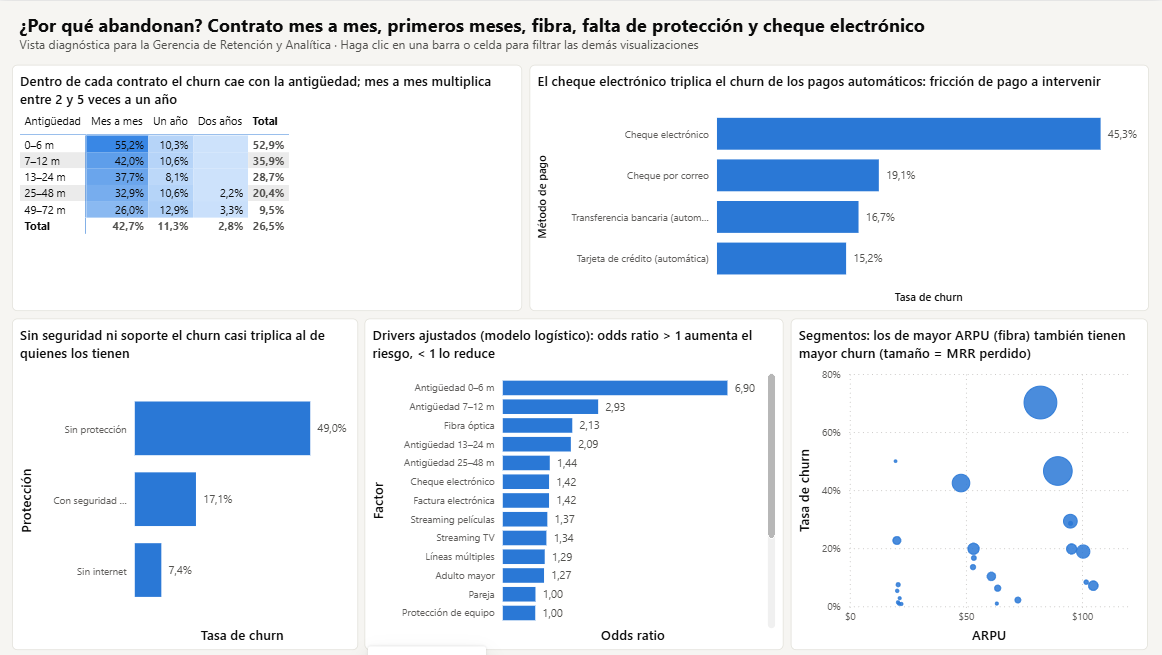
\includegraphics[width=0.92\textwidth]{dashboard_p2.png}
\caption{Página 2 · Diagnóstico.}
\end{figure}
\begin{figure}[H]
\centering
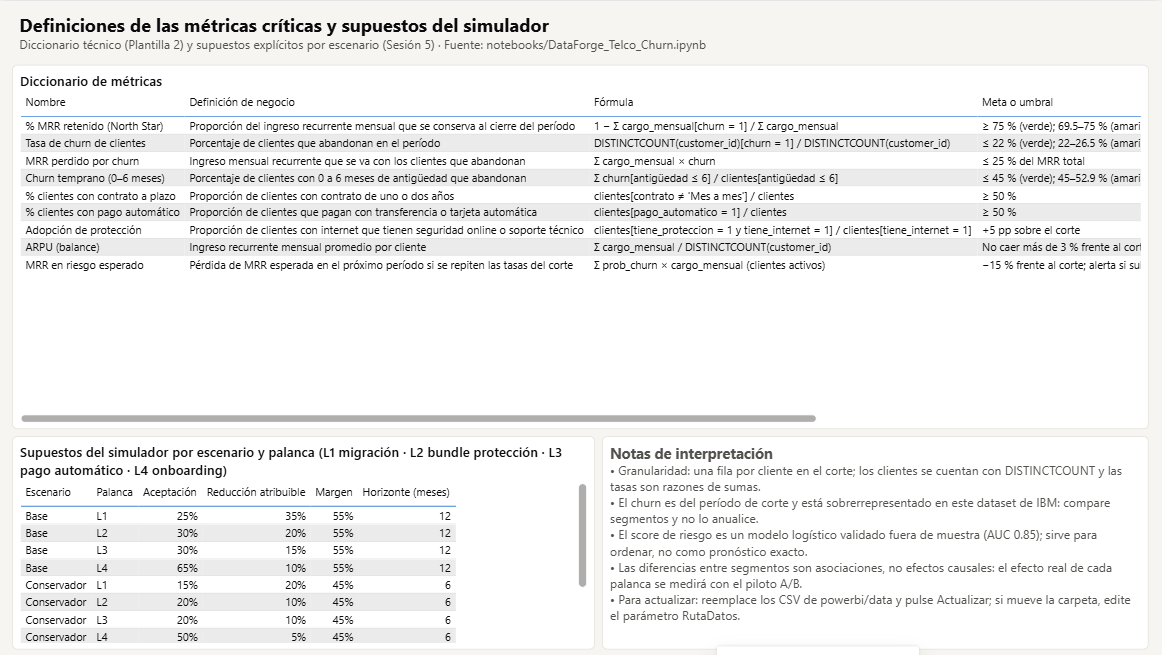
\includegraphics[width=0.92\textwidth]{dashboard_p4.png}
\caption{Página 4 · Definiciones y supuestos.}
\end{figure}
\textbf{Navegación.} Abrir \texttt{powerbi/DataForge\_Telco\_Churn.pbip} en Power BI Desktop y pulsar \emph{Actualizar} la primera vez. Los segmentadores de la página 1 filtran contrato, internet, pago y antigüedad. En la página 2, un clic en una barra o celda filtra el resto de visuales. En la página 3, el segmentador de escenario recalcula el ROI y la regla de decisión.

\section{Validación del score de riesgo}
\begin{figure}[H]
\centering
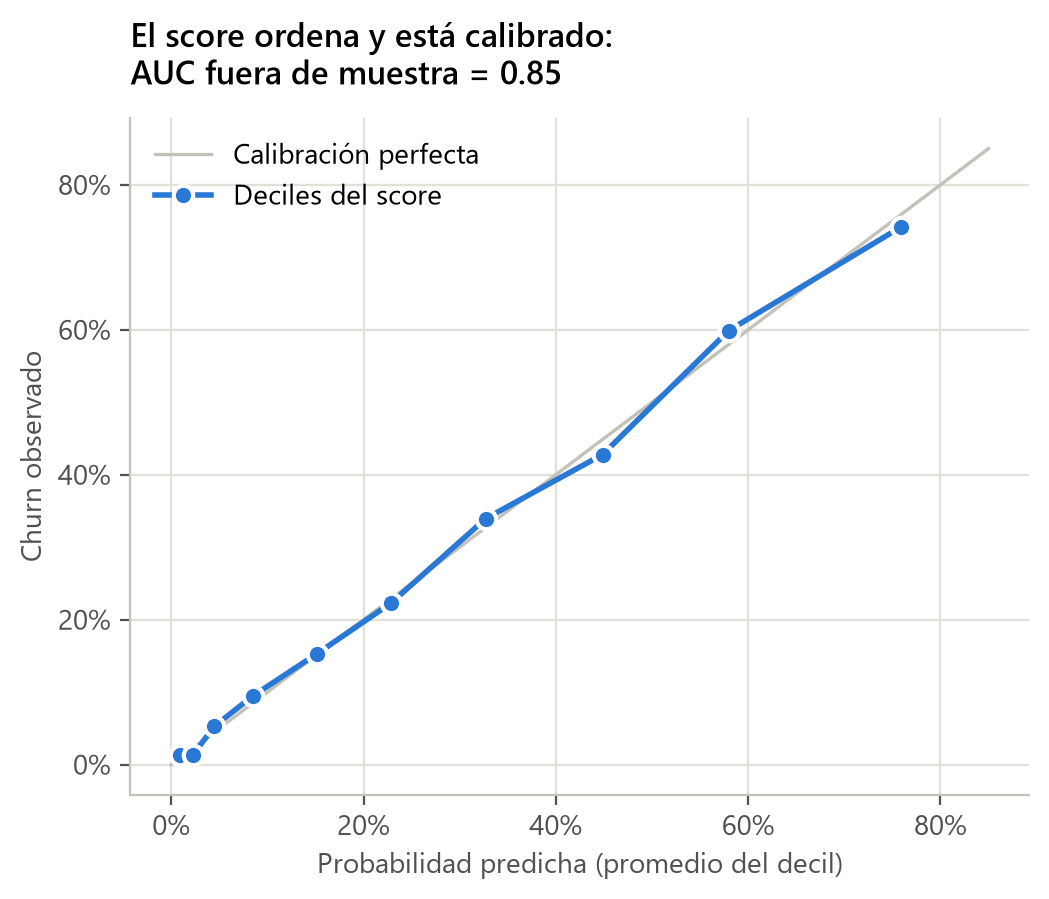
\includegraphics[width=0.45\textwidth]{f06_calibracion_score.png}
\caption{Calibración por deciles del score fuera de muestra (AUC = 0.85).}
\end{figure}

\section{Reproducibilidad}
\begin{enumerate}
  \item \texttt{python -m venv .venv} y \texttt{pip install -r requirements.txt}.
  \item Ejecutar \texttt{notebooks/DataForge\_Telco\_Churn.ipynb} completo. Lee \texttt{Data/}, regenera \texttt{outputs/} (figuras, tablas, cifras clave), \texttt{powerbi/data/} y \texttt{docs/diccionario\_metricas.md}.
  \item Abrir \texttt{powerbi/DataForge\_Telco\_Churn.pbip}, ajustar el parámetro \texttt{RutaDatos} si el repositorio se movió y pulsar \emph{Actualizar}.
  \item Informe: \texttt{python informe/generar\_anexos.py} y \texttt{pdflatex informe\_final.tex} (dos veces) desde \texttt{informe/}.
\end{enumerate}

\section{Nota sobre el uso de herramientas de IA}
% Nota exigida por la sección 13 del enunciado. El equipo debe revisar y completar lo que está entre corchetes antes de entregar.
\textbf{Herramienta y uso.} El equipo usó \textbf{Claude} (Anthropic), un asistente de IA, de forma sustancial para:
\begin{itemize}
  \item organizar el proyecto según el enunciado y el material de las sesiones 1 a 8;
  \item escribir y depurar el código del notebook (auditoría, limpieza, métricas, modelo logístico, simulación de ROI y diseño del piloto);
  \item generar el modelo semántico y el reporte de Power BI (TMDL y PBIR), incluidas las medidas DAX;
  \item redactar borradores del informe y de la presentación ejecutiva.
\end{itemize}

\textbf{Controles automáticos incluidos.} El notebook se ejecuta de principio a fin y contiene validaciones (\texttt{assert}) de llave única, ausencia de nulos, reconciliación del MRR y de los churners con el archivo crudo, tasas en [0, 1] e integridad referencial del modelo estrella. Las cifras del dashboard se contrastaron con las del notebook: NSM 69.5\,\%, MRR perdido USD 139 mil y ROI focalizado +179\,\%.

\textbf{Verificación y decisiones del equipo.} [Completar por el equipo: qué partes revisó cada integrante (por ejemplo, reglas de limpieza, fórmulas del diccionario, supuestos del simulador, lectura de los resultados), qué cambió respecto a la propuesta de la herramienta y qué decisiones tomó el equipo (por ejemplo, la elección del dataset, el usuario de la decisión, la North Star, los umbrales y la recomendación final).]

El equipo es responsable de todo el contenido entregado y puede explicar y defender cada análisis, supuesto y recomendación.


\end{document}
